\errorcontextlines9999
\documentclass[parskip=half,english,noenddot,numbers=noenddot,footnotes=nomultiple,oneside]{scrartcl}

\usepackage[T1]{fontenc}
\usepackage[utf8]{inputenc}
\usepackage[english]{babel}

\usepackage[glows]{tikzpingus}
\usepackage[linkcolor=pingu@purple,urlcolor=pingu@purple,colorlinks,breaklinks,pdfusetitle]{hyperref}
\urlstyle{same}
\expandafter\def\expandafter\UrlBreaks\expandafter{\UrlBreaks\do-}

\usepackage[tex,hyper]{listings}
\usepackage[most]{tcolorbox}
\usepackage{imakeidx,tikz,fontawesome,csquotes,enumitem,microtype,tikzducks,datatool,relsize,multicol,footnotebackref,adjustbox}
\makeindex[title={Key Overview},columns=2,columnsep=.75cm,noautomatic=true]
\deffootnote{1.5em}{1em}{\textsuperscript{\hyperref[\BackrefFootnoteTag]{\thefootnotemark}}\thinspace}
\def\thefootnote{$\langle$\arabic{footnote}$\rangle$}

\newlist{inlist}{enumerate*}{1}
\setlist[inlist]{itemjoin={{,\space}},itemjoin*={{, and }},label=$\roman*$),mode=boxed}
\let\say\enquote
\def\DTLlistformatoxford{,}
\def\DTLandname{and}
\def\DTLlistformatitem#1{\textit{#1}}
\newcommand*\typesetselection[1][]{\begingroup\ifx!#1!\else\def\DTLlistformatitem##1{#1}\fi\dotypesetselection}
\def\dotypesetselection#1{\expandafter\DTLformatlist\expandafter{\csname @pingu@#1@\endcsname}\endgroup}
\usepackage{lmodern,CrimsonPro}
\makeatletter

\addtokomafont{sectioning}{\color{gray}}
\addtokomafont{title}{\color{pingu@purple}}
\addtokomafont{author}{\normalsize}
\addtokomafont{date}{\normalsize}

\def\optstyle{\color{pingu@blue!75!black}\slshape}
\def\lstfnsize{-.7}
\lstdefinestyle{lstpingu}{%
	tabsize=2, breaklines,
	basicstyle=\relsize{\lstfnsize}\ttfamily,
	commentstyle={\color{gray}\slshape},
	columns=fullflexible,
	emphstyle=\slshape,
	emphstyle=[2]\optstyle,
	emphstyle=[3]\color{gray!75!white},
	emphstyle=[4]\color{pingu@blue!40!black},
	texcsstyle=*\color{gray}\bfseries,
	texcsstyle=*[2]\color{pingu@purple}\bfseries,
	texcsstyle=*[3]\color{gray!60!white},
	lineskip=2.75pt,
	keepspaces=true,
	moredelim=[s][\itshape]{<}{>},
}
\lstset{style=lstpingu}
\def\ipingu#1{\lstinline'#1'}
\def\lpingu#1{\lstinline[style=lstpingu,language=pingulang]'#1'}

\def\t@lst@addToLiterate#1{\protected@edef\lst@literate{\unexpanded\expandafter{\lst@literate}\unexpanded{#1}}}
\lst@Key{add to literate}{}{\t@lst@addToLiterate{#1}}

\lstdefinelanguage{pingulang}{
	language={[LaTeX]TeX},
	moreemph={tikzpicture},
	alsoletter={.-!:0123456789},%disable number
	moreemph=[2]{left,right,wing,eye,wings,tie,bow,none,eyes,shiny,wink,wave,grab,hug,wave,cup,straw,xshift,yshift,meta,dots,name,heart,shock,bill,hair,hairstyle,feet,foot,simple,flat,angry,back,devil,normal,princess,crown,silver,medal,patch,halo,glow,thick,2d,sunglasses,gem,shade,round,lollipop,lightsaber,item,angle,raise,cane,flip,flag,sign,post,cloak,scale,meta-dots,color,body,head,main,front,second,height,small,size,large,style,hairs,1,2,3,4,5,knot,length,offset,width,pattern,bowtie,bow-tie,a,b,text,gold,bronze,band,eyepatch,eye-patch,monocle,glass,opacity,string,blob,pants,button,buttons,bands,no,without,extra,steps,function,solid,right,frame,eye-frame,eyeframe,glasses,fill,line,sun,horns,devilhorns,devil-horns,headband,head-band,bend, upper,rook,hatch,strawhat,hat,ribbon,position,base,coronal,3d,colors,ring,bobbles,cake-hat,candle,fire,wick,outline,top,handle,hand,cast,handcast,signpost,font,fontcolor,deco,ribbs},
	moreemph=[4]{:line,:ghost,parts,:devil,:back},
	deletetexcs={begin,end},
	moretexcs=[2]{pingu,duck,node,pingudefaults,pingudefaultsappend},
	moretexcs=[3]{begin,end},
	moreemph=[3]{!hide,.style},
	add to literate={/pingu/}{{\textcolor{gray}{/pingu/}}}7
		{\{tikzpicture\}}{{\textcolor{gray!60!white}{\{tikzpicture\}}}}{13}
}
\NewEnviron{scaleme}[1]{\scalebox{#1}{\BODY}}

\RedeclareSectionCommand[runin=false,afterskip=-2mm]{section}

\tcbset{%
	colframe=gray,enhanced,breakable,
	arc=2mm, arc is angular,
	fonttitle=\bfseries,
	sidebyside,
	listing options={style=lstpingu,language=pingulang},
	center lower,
	righthand width=4.75cm,
	bottom=0pt,top=0pt,boxsep=2.25pt,
	before lower app={\parskip.5cm}
}
\lstMakeShortInline[style=lstpingu,basicstyle=\relsize{-1}\ttfamily\color{black!90!white}]{|}

\def\explaincolor{pingu@purple!8!white}
\def\cursub{}
\def\keyexplainindent{2em}%
\newenvironment{keyexplain}[4][/pingu/]{\begin{minipage}{\linewidth}%
	\parskip\medskipamount
	\phantomsection\label{pk:#1#2}\index{\cursub#2?\hyperref[pk:#1#2]{\protect\lpingu{#2}}}%
	\expandafter\gdef\csname pinguopt#2\endcsname{#3}%
	\expandafter\gdef\csname pingudefa#2\endcsname{#4}%
	\begingroup\pgfkeys{/pingu/.cd,defaults}\protected@edef\@tmp{#4}%
	\protected@edef\@tmpb{#3}%
	\hspace*{-\keyexplainindent}\colorbox{\explaincolor}{%
		\parbox{\dimexpr\linewidth-2\fboxsep+\keyexplainindent}{\small%
		\ifx\@tmpb\@empty\lpingu{#1#2}\else\lpingu{#1#2 =\ }\texttt{<\textit{\@tmpb}>}\fi\hfill
				\ifx\@tmp\@empty\else\textcolor{gray}{(}#4\textcolor{gray}{)}\fi%
		}
	}\\*[\smallskipamount]\endgroup}
{\end{minipage}\medskip\par}

\def\singleshortcut#1#2#3#4{\def\cursub{#2?\hyperref[pk:#1#2]{\protect\lpingu{#2}}!}\begin{keyexplain}[#1]{#2 #3}{\csname pinguopt#4\endcsname}{\csname pingudefa#4\endcsname}%
	\textcolor{gray}{\footnotesize This is a shortcut for: \texttt{\keyref[#1]{#2} = {\optstyle#3}}. The \enquote{\texttt{\textit{\csname pinguopt#4\endcsname}}} argument is passed to \keyref[#1]{#4}.}
\end{keyexplain}}
\newcommand*\shortcuts[4][/pingu/]{\begingroup
\protected@edef\@tmp{#3}%
\def\explaincolor{gray!10!white}%
\foreach \type in \@tmp {%
\edef\tmp{\noexpand\singleshortcut{#1}{#2}{\type}{#4}}\tmp
}\endgroup}

\newcommand*\keyref[2][/pingu/]{\hyperref[pk:#1#2]{\lpingu{#1#2}}}
\newenvironment{subkeyexplain}[5][/pingu/]{%
\begingroup
\def\explaincolor{gray!10!white}\def\keyexplainindent{0em}%
\def\cursub{#2?\hyperref[pk:#1#2]{\protect\lpingu{#2}}!}%
\begin{keyexplain}[#1]{#3}{#4}{#5}%
	\textcolor{gray}{\footnotesize This command is only in effect if \keyref[#1]{#2} is active.}\newline
}{\end{keyexplain}\endgroup}

\newcommand\keyalias[3][/pingu/]{\begingroup
\def\explaincolor{gray!10!white}\def\keyexplainindent{0em}%
\def\cursub{#3?\hyperref[pk:#1#3]{\protect\lpingu{#3}}!}%
\begin{keyexplain}[#1]{#2}{\csname pinguopt#3\endcsname}{\csname pingudefa#3\endcsname}%
	\textcolor{gray}{\footnotesize This is an alias for \keyref[#1]{#3}.}%
\end{keyexplain}\endgroup}
\newcommand\subkeyalias[4][/pingu/]{\begingroup
\def\explaincolor{gray!10!white}\def\keyexplainindent{0em}%
\def\cursub{#4?\hyperref[pk:#1#4]{\protect\lpingu{#4}}!#3?\hyperref[pk:#1#3]{\protect\lpingu{#3}}!}%
\begin{keyexplain}[#1]{#2}{\csname pinguopt#3\endcsname}{\csname pingudefa#3\endcsname}%
	\textcolor{gray}{\footnotesize This is an alias for \keyref[#1]{#3}.}%
\end{keyexplain}\endgroup}

\def\TikZ{Ti\textit{k}Z}
\def\tikzpingus{\TikZ pingus}

\title{The \texorpdfstring{\tikzpingus}{tikzpingus} package}
\subtitle{penguins in \TikZ}
\author{%
	\texorpdfstring{Florian Sihler\\[.4em]
		\url{https://github.com/EagleoutIce/tikzpingus}
	}{Florian Sihler}}
\date{Version v1.0 \textendash\ 2021/07/02}

\begin{document}
\maketitle

\section{Motivation}

For my slides at university, I started to use the fairly famous \LaTeX-package \textsl{\href{https://github.com/samcarter/tikzducks}{tikzducks}} a few years ago.
Yet, it seemed somewhat of a necessity to extend the range of available \say{cute} animals in \LaTeX.
Therefore I started writing this package: \textsl{tikzpingus}.\footnote{Why \say{pingu} and not \say{pengu}? Well, this is the third try on achieving cute penguins without using any templates or vector formats as a basis. As a german, the short form \say{pingu} was merely a typo that originated from the german word \say{pinguin} for \say{penguin}. It somewhat sticked\ldots}

\textit{Please note:} While tikzpingus is certainly inspired by tikzducks, it does offer a different set of features (e.g. multiple arm positions,~\ldots).

I would be happy for any feedback or issues on the \href{https://github.com/EagleoutIce/tikzpingus}{tikzpingus}-GitHub.

\subsection{Dependencies}

As this package is constantly work in progress, the concrete dependencies may change any time.
At the moment, it only loads \TikZ, which loads a lot of other packages (e.g. |xcolor|).
Furthermore, the following \TikZ-Libraries are in use:\footnote{A lot of the libraries loaded are important only for specific extras. I plan on cleaning them up.}
\begin{inlist}
	\item |intersections|
	\item |shadings|
	\item |patterns.meta|
	\item |decorations.pathmorphing|
	\item |shapes.symbols|
\end{inlist}.

\subsection{Copyright}

Copyright \textcopyright\ \texttt{Florian Sihler}. Permission is granted to copy, distribute and\slash or modify this software under the terms of the LaTeX project public licence, version 1.3c or later \url{http://www.latex-project.org/lppl.txt}.

The shown example penguins are purely fictional characters, any resemblance to real penguins or persons is purely coincidental and no copyright infringement is intended.

\section{Usage}

If you just want a penguin, use the following syntax:
\begin{tcblisting}{title={One small penguin}}

\begin{tikzpicture}
	\pingu
\end{tikzpicture}
\end{tcblisting}

There are \textit{a lot} of configuration-options which can be passed as an optional argument via the known |<key>=<value>|-style.
% TODO: click reference to full list; TODO: glow option
\begin{tcblisting}{title={Happy penguin with cup!}}
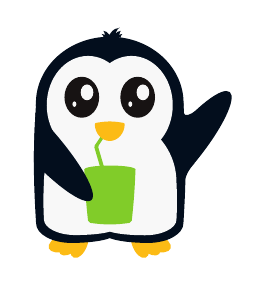
\begin{tikzpicture}
	\pingu[left wing wave, right wing grab,
	       eyes shiny, cup]
\end{tikzpicture}
\end{tcblisting}
Please note, that \say{left} and \say{right} have been chosen from the penguin-perspective.

Besides the keys defined by this package, you can use the keys of \TikZ\ and |pgf| as well (the duck was generated by the lovely \href{https://github.com/samcarter/tikzducks}{tikzducks} package):
\begin{tcblisting}{title={The Reunion}}
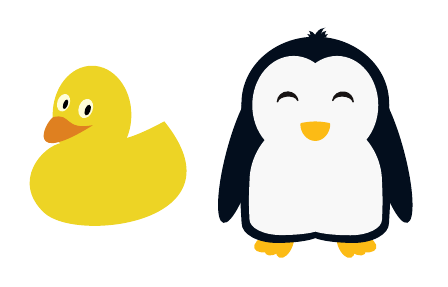
\begin{tikzpicture}
	\duck
	\pingu[xshift=2.8cm, yshift=14mm,
	       eyes wink]
\end{tikzpicture}
\end{tcblisting}
\subsection{Using the Coordinates}
\label{mrk:coordinates}While there are a lot of gadgets available already,
every penguin is accompanied by \textit{a lot} of adaptive coordinates
to place custom items, texts,~\ldots\ % TODO: links
They can be placed by the meta-dots option and change their positions, angles,~\ldots\ depending on other options.
Furthermore, some extras create further coordinates themselves!
All coordinates are available with |<pigu-name>-<coordinate>|.
While the default name of a penguin is \say{pingu}, it can be
changed with the name option:
\begin{tcblisting}{title={Lotta dots}}
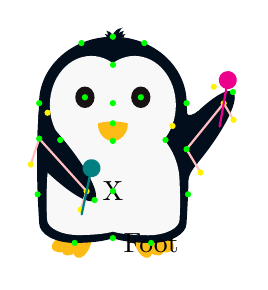
\begin{tikzpicture}
	\pingu[meta dots,left wing wave,
	       right wing grab, name=paula]
	\node at (paula-belly-center) {X};
	\node at (paula-foot-left) {Foot};
\end{tikzpicture}
\end{tcblisting}
Lets look at those coordinates in more detail (all labels are to be prefixed by |<pingu-name>-|):
\newsavebox\pinguwingright
\savebox\pinguwingright{%
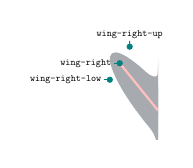
\begin{tikzpicture}%
	\scope
	\path[clip] (0,-.7) rectangle (-1,.7);
	\pgfonlayer{foreground}\path[clip] (0,-.7) rectangle (-1,.7);\endpgfonlayer
	\pingu[@block/.append style={fill=#1!35!white}, wings wave,eyes shiny,heart=gray!30!white,feet=none]
	\path[draw,pink,thick] (pingu-wing-right-start) -- (pingu-wing-right);
	\endscope
	\foreach \c/\a in {wing-right/left,wing-right-low/left,wing-right-up/above} {
		\path[fill=teal] (pingu-\c) circle [radius=1.125pt];
		\node[\a=.75mm,font=\ttfamily,scale=.35,inner sep=2.5pt] (expl-\c) at (pingu-\c) {\c};
		\draw[teal,thin] (expl-\c) -- (pingu-\c);
	}
\end{tikzpicture}}
\makeatletter
\newsavebox\pinguwingleft
\savebox\pinguwingleft{%
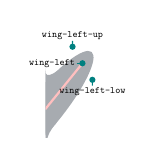
\begin{tikzpicture}%
	\scope
	\path[clip] (\pingu@w@half*2,-.7) rectangle ++(1,1.4);
	\pgfonlayer{foreground}\path[clip] (\pingu@w@half*2,-.7) rectangle ++(1,1.4);\endpgfonlayer
	\pingu[@block/.append style={fill=#1!35!white}, wings wave,eyes shiny,heart=gray!30!white,feet=none]
	\path[draw,pink,thick] (pingu-wing-left-start) -- (pingu-wing-left);
	\endscope
	\foreach \c/\a in {wing-left/left,wing-left-low/below,wing-left-up/above} {
		\path[fill=teal] (pingu-\c) circle [radius=1.125pt];
		\node[\a=.75mm,font=\ttfamily,scale=.35,inner sep=1.5pt] (expl-\c) at (pingu-\c) {\c};
		\draw[teal,thin] (expl-\c) -- (pingu-\c);
	}
\end{tikzpicture}%
}

\begin{center}
	\resizebox{.9\linewidth}!{
		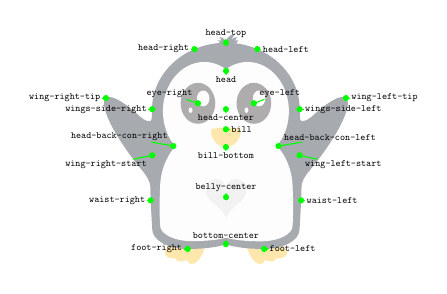
\begin{tikzpicture}
			\pingu[@block/.append style={fill=#1!35!white}, wings wave,eyes shiny,heart=gray!30!white]
			\pgfonlayer{foreground}
			\foreach \c/\a in {belly-center/above,head/below,head-top/above,foot-left/right,foot-right/left,eye-right/above left,eye-left/above right,bill/right,bill-bottom/below,wings-side-left/right,wings-side-right/left,wing-left-start/below right,wing-left-tip/right,wing-right-start/below left,wing-right-tip/left,head-right/left,head-left/right,head-center/below,head-back-con-left/above right,head-back-con-right/above left,bottom-center/above,waist-left/right,waist-right/left} {
				\path[fill=green] (pingu-\c) circle [radius=1.125pt];
				\node[\a=.5mm,font=\ttfamily,scale=.35,inner sep=1.5pt] (expl-\c) at (pingu-\c) {\c};
				\draw[green,thin] (expl-\c) -- (pingu-\c);
			}
			\endpgfonlayer
		\end{tikzpicture}
	}
\end{center}

\paragraph{The Wings}
This view excluded a lot of special data collected on the wings!
While there is more information stored for each wing, the following three coordinates are the most important to place items into penguins hand:
\begin{center}
	\null\hfill\parbox[c]{2.5\wd\pinguwingright}{\scalebox{2.5}{\usebox\pinguwingright}}\hfill\parbox[c]{4cm}{\centering\scriptsize\color{gray}\sffamily And yes, the wings are deliberately placed asymmetrical.\endgraf}\hfill
	\parbox[c]{2.5\wd\pinguwingleft}{\scalebox{2.5}{\usebox\pinguwingleft}}\hfill\null
\end{center}

\subsection{Colors}
A lot of options allow for a color to passed. In general, you can provide any color that \TikZ\ is happy with! Yet, there are some predefined pingu-colors shipped with this package, and there is one special \say{color}:
\begin{multicols}{4}
\begin{itemize}
	\foreach \col in {main,black,silver,bronze,white,yellow,lightblue,blue,green,red,purple} {
		\item[{\tikz[baseline=-.6ex]{\fill[pingu@\col,semithick,draw=black] circle (4pt);}}] \small\texttt{pingu@\col}
	}
	\item[] % buffer
\end{itemize}
\end{multicols}
Furthermore, there is the color {\makeatletter\say{\expandafter\ipingu\expandafter{\@pingu@none}}} which is available for most\footnote{Why just \say{most}? Well, this package is work in progress and I have added the option late, so I may have forgotten to patch some keys.} extras and wing-items. This color prohibits the compartments from being drawn. To be more precise, the package defines the macro |\pingu@none|, which is matched against the selected color.

As an example, lets take a look at the \keyref{cup}-extra, which provides an additional key \keyref{cup straw} to color the straw:
\begin{tcblisting}{title={Cup without a straw}}
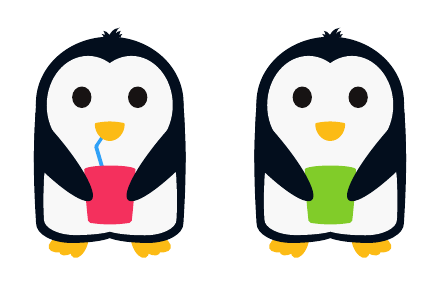
\begin{tikzpicture}
	\pingu[wings grab, cup=pingu@purple,
	       cup straw=pingu@blue]
	\pingu[wings grab, cup, xshift=2.8cm,
	       cup straw=!hide]
\end{tikzpicture}
\end{tcblisting}

\subsection{Setting the defaults}
You do not have to state every key for every penguin.
With the two macros \lstinline[language=pingulang]'\pingudefaults' and \lstinline[language=pingulang]'\pingudefaultsappend' (works the same, but will extend the current options) you can set default-options for all penguins to come:
\begin{tcblisting}{title={Change the mainstream}}
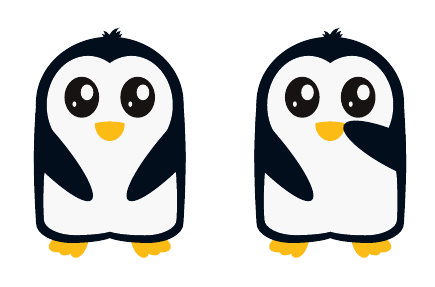
\begin{tikzpicture}
	\pingudefaults{wings grab, eyes shiny}
	\pingu
	\pingu[left wing shock, xshift=2.8cm]
\end{tikzpicture}
\end{tcblisting}

\subsection{Changing the wings}
\label{subsec:wings}As already demonstrated, it is possible to change the wing positions!
All selected wing-items will adapt to the wing-position (although not all wing-items will make sense with every wing-position).
Currently, there are the following wing-positions:
\typesetselection{leftwing}. \say{none} is a special wing-position: it omits the drawing of wings (teaser: every selection has a none-option, which prohibits the part from being drawn)!

For each valid wing-position you can use |wings <position>| to change both wings or |left wing <position>| and |right wing <position>| to change only one wing respectively. The default wing-position is \say{normal}. If you supply more than one option for a wing, only the last one will survive.\footnote{For the sake of completeness: \ipingu{wings <position>}, \ipingu{left wing <position>}, and \ipingu{right wing <position>} are just alternatives that i prefer over the underlying mechanism: \ipingu{wings=<position>}, \ipingu{left wing=<position>} and \ipingu{right wing=<position>}.}
\begin{tcblisting}{sidebyside=false, title=Wing-Showcase}
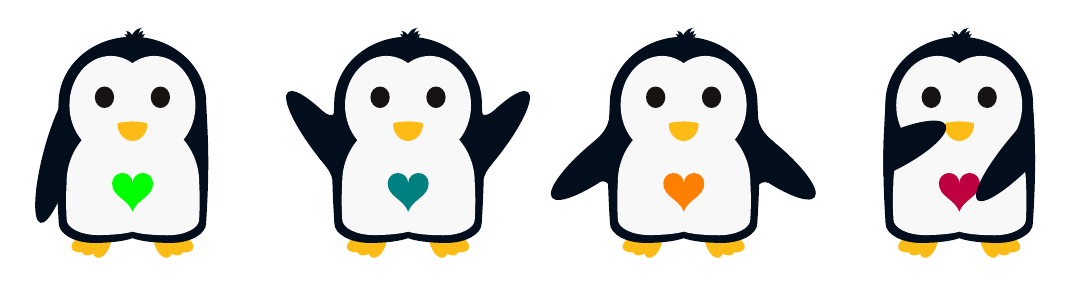
\begin{tikzpicture}
	\pingu[left wing none, heart=green]
	\pingu[wings wave, heart=teal, xshift=3.5cm]
	\pingu[wings hug, heart=orange, xshift=7cm]
	\pingu[left wing grab, right wing shock, heart=purple,  xshift=10.5cm]
\end{tikzpicture}
\end{tcblisting}

\subsection{Changing the eyes}
\label{mrk:pengu-eye}Just like the wings, there are a couple of different eye-styles to choose from: \typesetselection{lefteye}. Just like the wings, there is a \say{none} and a \say{normal}-option (which is the default).
Furthermore, the convenient selectors |eyes <style>|, |left eye <style>|, and |right eye <style>| exist as well:
\begin{tcblisting}{sidebyside=false, title=Eye-Showcase}
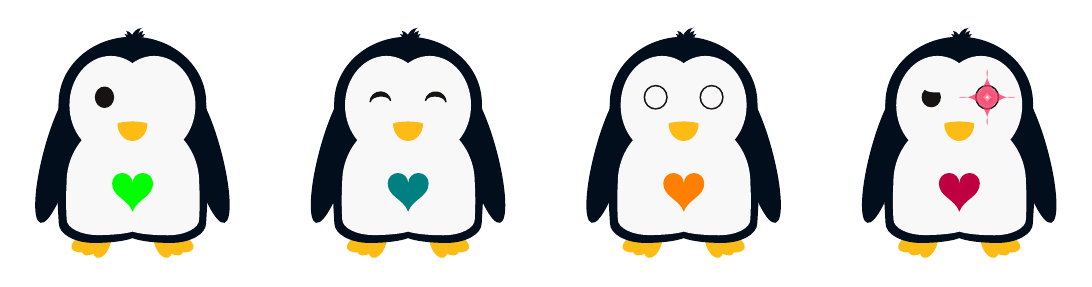
\begin{tikzpicture}
	\pingu[left eye none, heart=green]
	\pingu[eyes wink, heart=teal, xshift=3.5cm]
	\pingu[eyes shock, heart=orange, xshift=7cm]
	\pingu[left eye devil, right eye angry, heart=purple,  xshift=10.5cm]
\end{tikzpicture}
\end{tcblisting}

\subsection{Changing other components}
\label{mrk:pengu-change-comps}Just like for the wings and the eyes, you can change th following body parts:
\begin{itemize}
	\item The \textit{feet} (again with separate left and right)\\*
		Select from: \typesetselection{leftfoot}.
	\item The \textit{bill} (does not have left and right, as there is just one)\\*
		Select from: \typesetselection{bill}.
	\item The \textit{hairstyle} (does not have left and right)\\*
		Select from: \typesetselection{hairstyle}.
\end{itemize}
For each selection, \say{none} will prohibit the drawing, and \say{normal} is the default chosen.
\begin{tcblisting}{sidebyside=false, title=Bodyparts-Showcase}
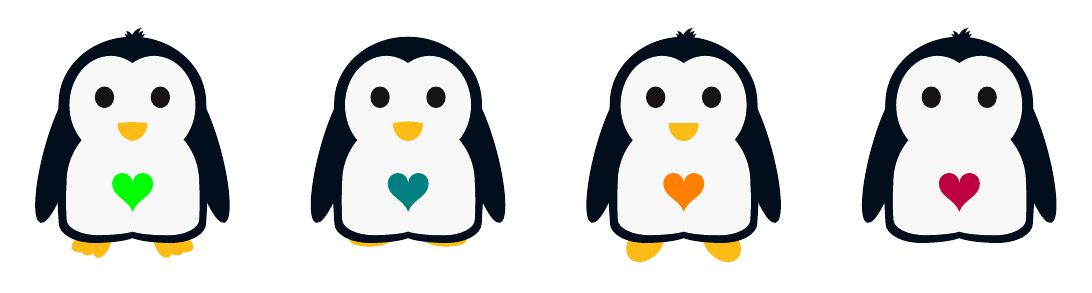
\begin{tikzpicture}
	\pingu[bill angry, heart=green]
	\pingu[feet back, hairstyle none, heart=teal, xshift=3.5cm]
	\pingu[bill flat, feet simple, heart=orange, xshift=7cm]
	\pingu[feet none, bill none, heart=purple, xshift=10.5cm]
\end{tikzpicture}
\end{tcblisting}

\subsection{Predefined Styles}
While the penguin options offer the modification of basically every drawing routine (through other styles like |@block|), it is tedious to change them every time.
So I have started to create some predefined styles, that do change some of the penguins appearance (and are completely new, so beware of bugs):
\begin{multicols}{2}
\begin{itemize}
	\foreach \tx/\s in {{draw everything with a line}/{:line}, {draw components with transparency}/{:ghost parts}, {draw all layers with transparency}/{:ghost}, {set all of the \say{devil}-components}/{:devil},{flip the penguin (swaps left \& right)}/{:back}} {
		\item \parbox[t]{.8\linewidth}{\raggedright\texttt{\s}, \tx.} \hfill
		\parbox[t]{.175\linewidth}{\scalebox{.4}{%
			
\begin{tikzpicture}[baseline=.35\baselineskip]%
				\pingu[\s]
			\end{tikzpicture}%
		}}
	}
	\item[] \parbox[t][2.4\baselineskip]{0pt}{}% buffer
\end{itemize}
\end{multicols}
Currently, only some of the styles do affect other items. As an example, consider |:line|, that changes the draw-style of wing-items and extras:
\begin{tcblisting}{title={Line Penguin}}
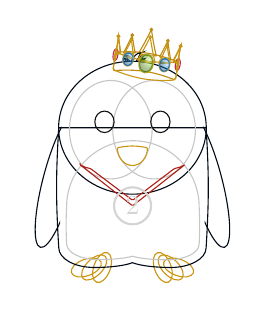
\begin{tikzpicture}
	\pingu[:line, princess crown, silver medal]
\end{tikzpicture}
\end{tcblisting}

\subsection{Extras}
An extra is considered everything, that is attached to the main penguin and not to the wings (as those items may be placed separately for both wings).
Most extras are activated with the format |<extra>=<color>| (the |<color>| option is not mandatory)
and try to adapt with other extras that have been placed (yet you can place multiple hats if you really like to).  A lot of the extras do offer more keys to customize their appearance.
They are explained in the full reference (\autoref{sec:full-ref}).

Consider the following, somewhat overkill-example:
\begin{tcblisting}{title={Lord-Gadget, the penguin}}

\begin{tikzpicture}
	\pingu[crown 2d=pingu@bronze,
	       medal=pingu@purple, tie,
	       eye patch left=teal,
	       eye patch right=orange,
	       right wing wave, sunglasses,
	       glow thick=yellow]
\end{tikzpicture}
\end{tcblisting}

\subsection{Wing-Items}
Wing items are basically just like extras, but they can be selected separately for the left and right wing. Furthermore, they adapt their \textit{default} appearance to the active wing positions (\autoref{subsec:wings}).
Currently there are the following wing items:
\typesetselection{wingitems}.
They are selected using |<wing item> <left/right>|.

Additionally, they can be customized by |<left/right> item angle=<angle>| and |<left/right> item flip=<true/false>|.
Lets consider an example\ldots
\begin{tcblisting}{title={Penguin with full wings!}}

\begin{tikzpicture}[scale=.75]
	\pingu[lightsaber right=orange,
	  lollipop left,
	  right item angle=70,
	  right wing raise, left wing grab]
	\pingu[cane left, right item flip,
	  sign post right={Hi!}, xshift=35mm]
\end{tikzpicture}
\end{tcblisting}

\subsection{Clothing}
Clothing is the newest extension to the collection, at and the moment there is not one \say{real} clothing, that really adapts to the penguins-position.
I am working on the \textit{cloak}-Clothing at the moment:
\begin{tcblisting}{title={Pengu-Clothes}}

\begin{tikzpicture}[scale=.75]
	\pingu[cloak]
\end{tikzpicture}
\end{tcblisting}

\section{Examples}

\appendix
\section{Full Reference}\label{sec:full-ref}

\begin{center}
	\textit{Please note, that all preview-penguins have been reduced in scale by \(40\,\%\) to save space and make the documentation more concise.}
\end{center}

Aliases my set custom defaults. Those defaults are not listed as they may change.

\def\lstfnsize{-1.65}
\tcbset{%
	before lower={\begin{adjustbox}{scale=.6}},
	after lower={\end{adjustbox}},%
	boxsep=0pt%
}

\subsection{Penguin Keys}
\begin{keyexplain}{name}{text}{\pingu@name}
	Sets the name of the penguin. This name is used for all the automatically generated coordinates (see \autoref{mrk:coordinates}).
\end{keyexplain}

\begin{keyexplain}{scale}{floating point}{active scale}
	Changes the scale for the penguin. This is not supported by all items by default (as some scales have to be re-calculated according to their rotation).
	Yet, it should work with most.

	Furthermore, this value can be used to make the penguin independent of the outer scaling.
\end{keyexplain}

\begin{keyexplain}{meta-dots}{true/false}{\if@pingu@draw@metadots true\else false\fi}
	Can be used to enable and disable the meta dots (\autoref{mrk:coordinates}).
	Passed true by default.
\end{keyexplain}

\keyalias{meta dots}{meta-dots}

\subsubsection{The Feet}

\begin{keyexplain}{left foot}{foot-selector}{\@pingu@select@leftfoot@}
	Change the style of the left foot. All valid values are listed in \autoref{mrk:pengu-change-comps}.
\begin{tcblisting}{listing options={style=lstpingu,language=pingulang,deleteemph={[2]{simple}}}}

\begin{tikzpicture}
	\pingu[left foot=simple]
\end{tikzpicture}
\end{tcblisting}
\end{keyexplain}

\begin{keyexplain}{left foot color}{color}{\pingu@color@foot@left}
	Change the color of the left foot of the penguin.%
\begin{tcblisting}{}
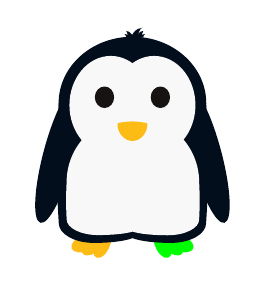
\begin{tikzpicture}
	\pingu[left foot color=green]
\end{tikzpicture}
\end{tcblisting}
\end{keyexplain}

\shortcuts{left foot}{\@pingu@leftfoot@}{left foot color}

\begin{keyexplain}{right foot}{foot-selector}{\@pingu@select@rightfoot@}
	Change the style of the right foot. All valid values are listed in \autoref{mrk:pengu-change-comps}.
\begin{tcblisting}{listing options={style=lstpingu,language=pingulang,deleteemph={[2]{simple}}}}

\begin{tikzpicture}
	\pingu[right foot=simple]
\end{tikzpicture}
\end{tcblisting}
\end{keyexplain}

\begin{keyexplain}{right foot color}{color}{\pingu@color@foot@right}
	Change the color of the right foot of the penguin.%
\begin{tcblisting}{}
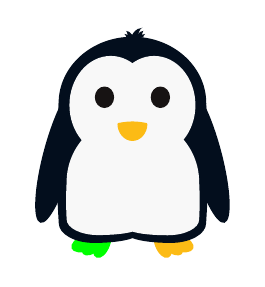
\begin{tikzpicture}
	\pingu[right foot color=green]
\end{tikzpicture}
\end{tcblisting}
\end{keyexplain}

\shortcuts{right foot}{\@pingu@rightfoot@}{right foot color}

\begin{keyexplain}{feet}{foot-selector}{}
	Change the style of both feet by calling \keyref{left foot} and \keyref{right foot} with the same value.
\begin{tcblisting}{listing options={style=lstpingu,language=pingulang,deleteemph={[2]{simple}}}}

\begin{tikzpicture}
	\pingu[feet=simple]
\end{tikzpicture}
\end{tcblisting}
\end{keyexplain}

\begin{keyexplain}{feet color}{color}{}
	Sets the color of both feet by calling \keyref{left foot color} and \keyref{right foot color} with the same value.
\begin{tcblisting}{}
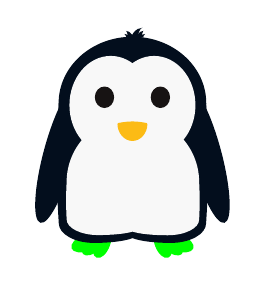
\begin{tikzpicture}
	\pingu[feet color=green]
\end{tikzpicture}
\end{tcblisting}
\end{keyexplain}

\shortcuts{feet}{\@pingu@leftfoot@}{feet color}

\subsubsection{The Body}
\begin{keyexplain}{body main}{color}{\pingu@color@body@main}
	Set the main color of the penguin. This will affect \keyref{hair} as well, as this chooses its default value from the main color.%
\begin{tcblisting}{}
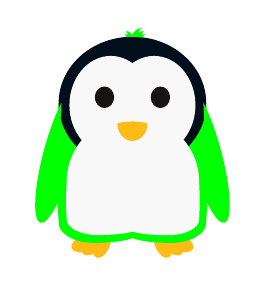
\begin{tikzpicture}
	\pingu[body main=green]
\end{tikzpicture}
\end{tcblisting}
\end{keyexplain}

\begin{keyexplain}{body head}{color}{\pingu@color@body@head}
	Set the color of the penguin head.%
\begin{tcblisting}{}
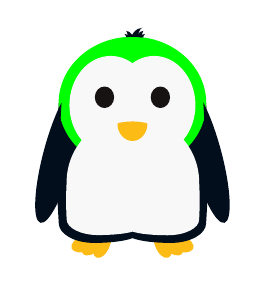
\begin{tikzpicture}
	\pingu[body head=green]
\end{tikzpicture}
\end{tcblisting}
\end{keyexplain}

\begin{keyexplain}{body}{color}{}
	Sets the color of the main penguin and the head, by calling \keyref{body main} and \keyref{body head} with the same value.
\begin{tcblisting}{}
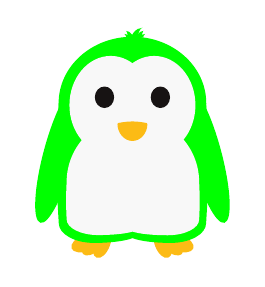
\begin{tikzpicture}
	\pingu[body=green]
\end{tikzpicture}
\end{tcblisting}
\end{keyexplain}

\begin{keyexplain}{body front}{color}{\pingu@color@body@front}
	Sets the frontal color of the penguin.
\begin{tcblisting}{}
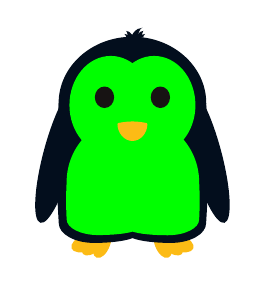
\begin{tikzpicture}
	\pingu[body front=green]
\end{tikzpicture}
\end{tcblisting}
\end{keyexplain}


\subsubsection{The Size}

\begin{keyexplain}{height}{length}{\the\pingu@side@h@half}
	Change the height of the penguin manually. You probably should not use this key directly and refer to \keyref{small size}, \keyref{normal size}, and \keyref{large size}:
\begin{tcblisting}{listing options={style=lstpingu,language=pingulang}}

\begin{tikzpicture}
	\pingu[height=17mm]
\end{tikzpicture}
\end{tcblisting}
\end{keyexplain}

\begin{keyexplain}{small size}{}{}
	Will use \keyref{height} to create a small pingu:
\begin{tcblisting}{listing options={style=lstpingu,language=pingulang}}

\begin{tikzpicture}
	\pingu[small size]
\end{tikzpicture}
\end{tcblisting}
\end{keyexplain}

\keyalias{small}{small size}
\keyalias{small height}{small size}

\begin{keyexplain}{normal size}{}{}
	Will use \keyref{height} to create a normal pingu:
\begin{tcblisting}{listing options={style=lstpingu,language=pingulang}}

\begin{tikzpicture}
	\pingu[normal size]
\end{tikzpicture}
\end{tcblisting}
\end{keyexplain}

\keyalias{normal}{normal size}
\keyalias{normal height}{normal size}

\begin{keyexplain}{large size}{}{}
	Will use \keyref{height} to create a large pingu:
\begin{tcblisting}{listing options={style=lstpingu,language=pingulang}}

\begin{tikzpicture}
	\pingu[large size]
\end{tikzpicture}
\end{tcblisting}
\end{keyexplain}

\keyalias{large}{large size}
\keyalias{large height}{large size}

\subsubsection{The Eyes}
\begin{keyexplain}{left eye}{eye-selector}{\@pingu@select@lefteye@}
	Change the style of the left eye. All valid values are listed in \autoref{mrk:pengu-eye}.
\begin{tcblisting}{listing options={style=lstpingu,language=pingulang,deleteemph={[2]{wink}}}}

\begin{tikzpicture}
	\pingu[left eye=wink]
\end{tikzpicture}
\end{tcblisting}
\end{keyexplain}

\begin{keyexplain}{left eye color}{color}{\pingu@color@eye@left}
	Change the main color of the left eye.
\begin{tcblisting}{}
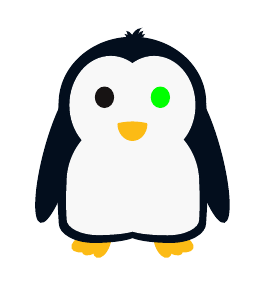
\begin{tikzpicture}
	\pingu[left eye color=green]
\end{tikzpicture}
\end{tcblisting}
\end{keyexplain}

\begin{keyexplain}{left eye second color}{color}{\pingu@color@eye@second@left}
	Change the secondary color of the left eye. It will be used in some styles selected by \keyref{left eye} (e.g. \textit{shiny}):
\begin{tcblisting}{listing options={style=lstpingu,language=pingulang,deleteemph={[2]{shiny}}}}
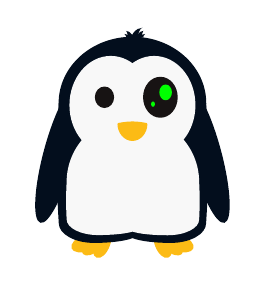
\begin{tikzpicture}
	\pingu[left eye=shiny,
	  left eye second color=green]
\end{tikzpicture}
\end{tcblisting}
\end{keyexplain}

\shortcuts{left eye}{\@pingu@lefteye@}{left eye color}

\begin{keyexplain}{right eye}{eye-selector}{\@pingu@select@righteye@}
	Change the style of the right eye. All valid values are listed in \autoref{mrk:pengu-eye}.
\begin{tcblisting}{listing options={style=lstpingu,language=pingulang,deleteemph={[2]{wink}}}}

\begin{tikzpicture}
	\pingu[right eye=wink]
\end{tikzpicture}
\end{tcblisting}
\end{keyexplain}

\begin{keyexplain}{right eye color}{color}{\pingu@color@eye@right}
	Change the main color of the right eye.
\begin{tcblisting}{}
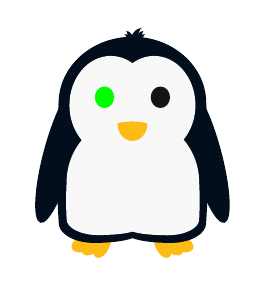
\begin{tikzpicture}
	\pingu[right eye color=green]
\end{tikzpicture}
\end{tcblisting}
\end{keyexplain}

\begin{keyexplain}{right eye second color}{color}{\pingu@color@eye@second@right}
	Change the secondary color of the right eye. It will be used in some styles selected by \keyref{right eye} (e.g. \textit{shiny}):
\begin{tcblisting}{listing options={style=lstpingu,language=pingulang,deleteemph={[2]{shock}}}}
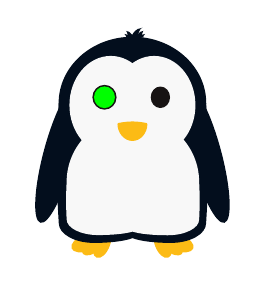
\begin{tikzpicture}
	\pingu[right eye=shock,
	  right eye second color=green]
\end{tikzpicture}
\end{tcblisting}
\end{keyexplain}

\shortcuts{right eye}{\@pingu@righteye@}{right eye color}

\begin{keyexplain}{eyes}{eye-selector}{}
	Change the style of both eyes by calling \keyref{left eye} and \keyref{right eye} with the same value.
\begin{tcblisting}{listing options={style=lstpingu,language=pingulang,deleteemph={[2]{wink}}}}

\begin{tikzpicture}
	\pingu[eyes=wink]
\end{tikzpicture}
\end{tcblisting}
\end{keyexplain}

\begin{keyexplain}{eyes color}{color}{}
	Change the main color of both eyes by calling \keyref{left eye color} and \keyref{right eye color} with the same value.
\begin{tcblisting}{}
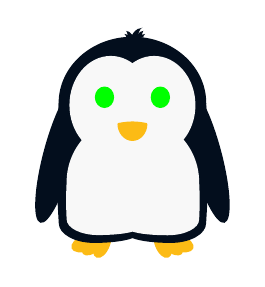
\begin{tikzpicture}
	\pingu[eyes color=green]
\end{tikzpicture}
\end{tcblisting}
\end{keyexplain}

\begin{keyexplain}{eyes second color}{color}{}
	Change the secondary color of  both eyes by calling \keyref{left eye second color} and \keyref{right eye second  color} with the same value.
\begin{tcblisting}{listing options={style=lstpingu,language=pingulang,deleteemph={[2]{shock,shiny}}}}
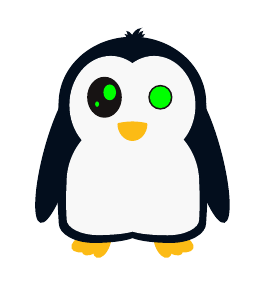
\begin{tikzpicture}
	\pingu[left eye=shock, right eye=shiny,
	  eyes second color=green]
\end{tikzpicture}
\end{tcblisting}
\end{keyexplain}

\shortcuts{eyes}{\@pingu@lefteye@}{eyes color}

\subsubsection{The Wings}

\begin{keyexplain}{left wing}{wing-selector}{\@pingu@select@leftwing@}
	Change the style of the left wing. All valid values are listed in \autoref{subsec:wings}.
\begin{tcblisting}{listing options={style=lstpingu,language=pingulang,deleteemph={[2]{wave}}}}

\begin{tikzpicture}
	\pingu[left wing=wave]
\end{tikzpicture}
\end{tcblisting}
\end{keyexplain}

\begin{keyexplain}{left wing color}{color}{\pingu@color@left@wing}
	Change the main color of the left wing.
\begin{tcblisting}{}
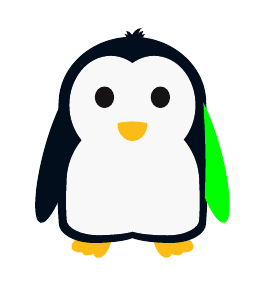
\begin{tikzpicture}
	\pingu[left wing color=green]
\end{tikzpicture}
\end{tcblisting}
\end{keyexplain}

\shortcuts{left wing}{\@pingu@leftwing@}{left wing color}

\begin{keyexplain}{right wing}{wing-selector}{\@pingu@select@rightwing@}
	Change the style of the right wing. All valid values are listed in \autoref{subsec:wings}.
\begin{tcblisting}{listing options={style=lstpingu,language=pingulang,deleteemph={[2]{wave}}}}

\begin{tikzpicture}
	\pingu[right wing=hug]
\end{tikzpicture}
\end{tcblisting}
\end{keyexplain}

\begin{keyexplain}{right wing color}{color}{\pingu@color@right@wing}
	Change the main color of the right wing.
\begin{tcblisting}{}
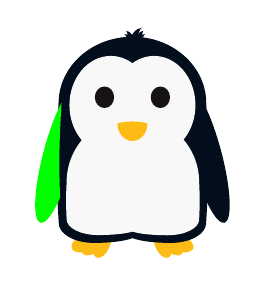
\begin{tikzpicture}
	\pingu[right wing color=green]
\end{tikzpicture}
\end{tcblisting}
\end{keyexplain}

\shortcuts{right wing}{\@pingu@rightwing@}{right wing color}

\begin{keyexplain}{wings}{wing-selector}{}
	Change the style of both wings by calling \keyref{left wing} and \keyref{right wing} with the same value.
\begin{tcblisting}{listing options={style=lstpingu,language=pingulang,deleteemph={[2]{wink}}}}

\begin{tikzpicture}
	\pingu[wings=grab]
\end{tikzpicture}
\end{tcblisting}
\end{keyexplain}

\begin{keyexplain}{wings color}{color}{}
	Change the main color of both wings by calling \keyref{left wing color} and \keyref{right wing color} with the same value.
\begin{tcblisting}{}
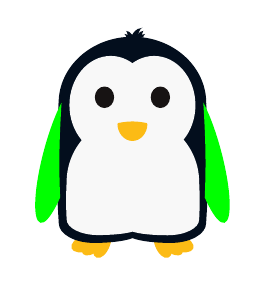
\begin{tikzpicture}
	\pingu[wings color=green]
\end{tikzpicture}
\end{tcblisting}
\end{keyexplain}

\shortcuts{wings}{\@pingu@leftwing@}{wings color}

\subsubsection{The Hair}
\begin{keyexplain}{hairstyle}{hair-selector}{\@pingu@select@hairstyle@}
	Change the hairstyle (\autoref{mrk:pengu-change-comps}):
\begin{tcblisting}{}

\begin{tikzpicture}
	\pingu[hairstyle=none]
\end{tikzpicture}
\end{tcblisting}
\end{keyexplain}

\keyalias{hair style}{hairstyle}
% \shortcuts{hair}{\@pingu@hairstyle@}{wings color}

\begin{keyexplain}{hair 1 color}{color}{\pingu@color@hair@a}
	Set the color of the first hair (this may be used differently by other hairstyles):
\begin{tcblisting}{listing options={style=lstpingu,language=pingulang,moreemph={[2]{1}}}}
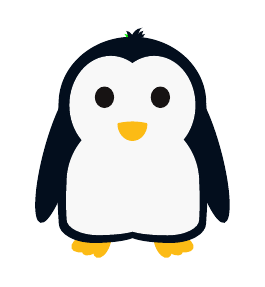
\begin{tikzpicture}
	\pingu[hair 1 color=green]
\end{tikzpicture}
\end{tcblisting}
\end{keyexplain}

\begin{keyexplain}{hair 2 color}{color}{\pingu@color@hair@b}
	Set the color of the second hair (this may be used differently by other hairstyles):
\begin{tcblisting}{listing options={style=lstpingu,language=pingulang,moreemph={[2]{2}}}}
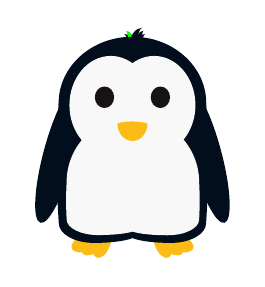
\begin{tikzpicture}
	\pingu[hair 2 color=green]
\end{tikzpicture}
\end{tcblisting}
\end{keyexplain}

\begin{keyexplain}{hair 3 color}{color}{\pingu@color@hair@c}
	Set the color of the third hair (this may be used differently by other hairstyles):
\begin{tcblisting}{listing options={style=lstpingu,language=pingulang,moreemph={[2]{3}}}}
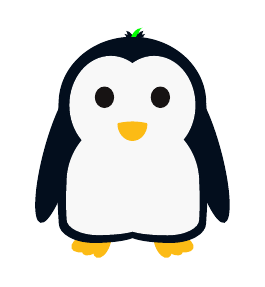
\begin{tikzpicture}
	\pingu[hair 3 color=green]
\end{tikzpicture}
\end{tcblisting}
\end{keyexplain}

\begin{keyexplain}{hair 4 color}{color}{\pingu@color@hair@d}
	Set the color of the fourth hair (this may be used differently by other hairstyles):
\begin{tcblisting}{listing options={style=lstpingu,language=pingulang,moreemph={[2]{4}}}}
\begin{tikzpicture}
	\pingu[hair 4 color=green]
\end{tikzpicture}
\end{tcblisting}
\end{keyexplain}

\begin{keyexplain}{hair 5 color}{color}{\pingu@color@hair@e}
	Set the color of the fifth hair (this may be used differently by other hairstyles):
\begin{tcblisting}{listing options={style=lstpingu,language=pingulang,moreemph={[2]{5}}}}
\begin{tikzpicture}
	\pingu[hair 5 color=green]
\end{tikzpicture}
\end{tcblisting}
\end{keyexplain}

\begin{keyexplain}{hairs color}{color}{}
	Set the color of all hairs by calling \keyref{hair 1 color}, \keyref{hair 2 color}, \keyref{hair 3 color}, \keyref{hair 4 color}, and \keyref{hair 5 color} with the same argument:
\begin{tcblisting}{}
\begin{tikzpicture}
	\pingu[hairs color=green]
\end{tikzpicture}
\end{tcblisting}
\end{keyexplain}

\keyalias{hairs}{hairs color}
\keyalias{hair}{hairs color}

\subsubsection{The Bill}
\begin{keyexplain}{bill}{bill-selector}{\@pingu@select@bill@}
	Change the style of the bill (\autoref{mrk:pengu-change-comps}):
\begin{tcblisting}{listing options={style=lstpingu,language=pingulang,deleteemph={[2]{flat}}}}
\begin{tikzpicture}
	\pingu[bill=flat]
\end{tikzpicture}
\end{tcblisting}
\end{keyexplain}

\begin{keyexplain}{bill color}{color}{\pingu@color@bill}
	Change the color of the bill
\begin{tcblisting}{}
\begin{tikzpicture}
	\pingu[bill color=green]
\end{tikzpicture}
\end{tcblisting}
\end{keyexplain}

\subsection{Drawing Styles}
\index{Styles}
\def\cursub{Styles!}
\begin{keyexplain}{:line}{}{}
	Disable glows, shades and fills and enforce a line. This line will be darker
	than the original fill color:
\begin{tcblisting}{}
\begin{tikzpicture}
	\pingu[:line]
\end{tikzpicture}
\end{tcblisting}
\end{keyexplain}

\begin{keyexplain}{:ghost parts}{opacity}{.5}
	Set the opacity of each penguin component individually. At the moment, this
	excludes some glow calculations.
\begin{tcblisting}{}
\begin{tikzpicture}
	\pingu[:ghost parts]
\end{tikzpicture}
\end{tcblisting}
\end{keyexplain}

\begin{keyexplain}{:ghost}{opacity}{.5}
	Set the opacity of the complete penguin. At the moment, this
	excludes some glow calculations.
\begin{tcblisting}{}
\begin{tikzpicture}
	\pingu[:ghost]
\end{tikzpicture}
\end{tcblisting}
\end{keyexplain}

\begin{keyexplain}{:devil}{color}{pingu@purple}
	Enable all devil components and set their main color:
\begin{tcblisting}{}
\begin{tikzpicture}
	\pingu[:devil=green]
\end{tikzpicture}
\end{tcblisting}
\end{keyexplain}

\begin{keyexplain}{:back}{}{}
	Mirror the penguin, this swaps left and right, the rotation and more.
	Yet, at least at the time of writing, this does not swap the drawing order in each layer, but just the layers:\typeout{KTWKKS}
\begin{tcblisting}{}
\begin{tikzpicture}
	\pingu[:back, left wing wave,
	       cane left, left item angle=70]
\end{tikzpicture}
\end{tcblisting}
\end{keyexplain}

\def\cursub{}

\subsection{Extras}

\subsubsection{The tie}
\begin{keyexplain}{tie}{color}{pingu@green}
	Enable the tie extra:
\begin{tcblisting}{}
\begin{tikzpicture}
	\pingu[tie]
\end{tikzpicture}
\end{tcblisting}
\end{keyexplain}

{\def\pingu@color@tie{<tie-color>}
\begin{subkeyexplain}{tie}{tie knot}{color}{\pingu@color@tie@knot}
	Change the tie knot:
\begin{tcblisting}{}
\begin{tikzpicture}
	\pingu[tie, tie knot=orange]
\end{tikzpicture}
\end{tcblisting}
\end{subkeyexplain}
}

\begin{subkeyexplain}{tie}{tie length}{length}{\expandafter\detokenize\expandafter{\pingu@x@tie@length}}
	Change the length of the tie:
\begin{tcblisting}{}
\begin{tikzpicture}
	\pingu[tie, tie length=1.25cm]
\end{tikzpicture}
\end{tcblisting}
\end{subkeyexplain}

\begin{subkeyexplain}{tie}{tie offset}{length}{\pingu@x@tie@offset}
	Change the upper vertical offset of the tie:
\begin{tcblisting}{}
\begin{tikzpicture}
	\pingu[tie, tie offset=.75cm]
\end{tikzpicture}
\end{tcblisting}
\end{subkeyexplain}

\begin{subkeyexplain}{tie}{tie width}{length}{\pingu@x@tie@width}
	Change the width of the tie:
\begin{tcblisting}{}
\begin{tikzpicture}
	\pingu[tie, tie width=.5cm]
\end{tikzpicture}
\end{tcblisting}
\end{subkeyexplain}

\begin{subkeyexplain}{tie}{tie pattern}{tex-code}{}
	Change the tie pattern.
\end{subkeyexplain}

\begin{subkeyexplain}{tie}{tie dots}{color}{pingu@white}
	Change the \keyref{tie pattern} to dots:
	\begin{tcblisting}{}
	\begin{tikzpicture}
		\pingu[tie, tie dots]
	\end{tikzpicture}
	\end{tcblisting}
\end{subkeyexplain}

\subsubsection{The bowtie}

\begin{keyexplain}{bow tie}{color}{pingu@blue}
	Enable the bow tie extra:
\begin{tcblisting}{}
\begin{tikzpicture}
	\pingu[bow tie]
\end{tikzpicture}
\end{tcblisting}
\end{keyexplain}

\keyalias{bowtie}{bow tie}
\keyalias{bow-tie}{bow tie}

\begin{subkeyexplain}{bow tie}{bow tie b}{color}{<bowtie-color>}
Change the color of the other bow-tie-wing:
\begin{tcblisting}{}
\begin{tikzpicture}
	\pingu[bow tie, bow tie b=green]
\end{tikzpicture}
\end{tcblisting}
\end{subkeyexplain}

\subkeyalias{bowtie b}{bow tie b}{bow tie}
\subkeyalias{bow-tie b}{bow tie b}{bow tie}

{\def\pingu@color@bowtie{<bowtie-color>}
\begin{subkeyexplain}{bow tie}{bow tie knot}{color}{\pingu@color@bowtie@knot}
change the color of the knot:
\begin{tcblisting}{}
\begin{tikzpicture}
	\pingu[bow tie, bow tie knot=green]
\end{tikzpicture}
\end{tcblisting}
\end{subkeyexplain}

\subkeyalias{bowtie knot}{bow tie knot}{bow tie}
\subkeyalias{bow-tie knot}{bow tie knot}{bow tie}
}

\begin{subkeyexplain}{bow tie}{bow tie offset}{length}{\pingu@x@bowtie@offset}
Change the vertical offset of the bow tie:
\begin{tcblisting}{}
\begin{tikzpicture}
	\pingu[bow tie, bow tie offset=8mm]
\end{tikzpicture}
\end{tcblisting}
\end{subkeyexplain}

\subkeyalias{bowtie offset}{bow tie offset}{bow tie}
\subkeyalias{bow-tie offset}{bow tie offset}{bow tie}

\subsubsection{The cup}
\begin{keyexplain}{cup}{color}{pingu@green}
	Change the color of the cup:
\begin{tcblisting}{}
\begin{tikzpicture}
	\pingu[cup]
\end{tikzpicture}
\end{tcblisting}
\end{keyexplain}

{\def\pingu@color@cup{<cup-color>}
\begin{subkeyexplain}{cup}{cup straw}{color}{\pingu@color@cup@straw}
Change the color of the cup straw
\begin{tcblisting}{}
\begin{tikzpicture}
	\pingu[cup, cup straw=!hide]
\end{tikzpicture}
\end{tcblisting}
\end{subkeyexplain}}

\subsubsection{The medal}
\begin{keyexplain}{medal}{color}{pingu@yellow}
	Change the color of the medal:
\begin{tcblisting}{}
\begin{tikzpicture}
	\pingu[medal]
\end{tikzpicture}
\end{tcblisting}
\end{keyexplain}

\begin{subkeyexplain}{medal}{medal band}{color}{\pingu@color@medal@band}
Change the color of the medal band:
\begin{tcblisting}{}
\begin{tikzpicture}
	\pingu[medal, medal band=green]
\end{tikzpicture}
\end{tcblisting}
\end{subkeyexplain}

{\def\pingu@color@medal{<medal-color>}
\begin{subkeyexplain}{medal}{medal shade}{color}{\pingu@color@medal@shade}
Change the color of the outer medal ring:
\begin{tcblisting}{}
\begin{tikzpicture}
	\pingu[medal, medal shade=green]
\end{tikzpicture}
\end{tcblisting}
\end{subkeyexplain}}

\begin{subkeyexplain}{medal}{medal shade width}{length}{.75pt}
Change the width of the outer medal ring:
\begin{tcblisting}{}
\begin{tikzpicture}
	\pingu[medal, medal shade=green,
	       medal shade width=2mm]
\end{tikzpicture}
\end{tcblisting}
\end{subkeyexplain}

\begin{subkeyexplain}{medal}{medal text}{text}{\pingu@x@medal@text}
Set the text displayed in the medal. The style can be changed by
updating the substyle \texttt{medal text style}.
\begin{tcblisting}{}
\begin{tikzpicture}
	\pingu[medal, medal text=XY,
	      medal text style/.style={black}]
\end{tikzpicture}
\end{tcblisting}
\end{subkeyexplain}

\begin{keyexplain}{gold medal}{text}{1}
Basically the same as the normal medal. This will activate \keyref{medal}:
\begin{tcblisting}{}
\begin{tikzpicture}
	\pingu[gold medal]
\end{tikzpicture}
\end{tcblisting}
\end{keyexplain}

\begin{keyexplain}{silver medal}{text}{2}
Basically the same as the normal medal, but with a silver color. This will activate \keyref{medal}:
\begin{tcblisting}{}
\begin{tikzpicture}
	\pingu[silver medal]
\end{tikzpicture}
\end{tcblisting}
\end{keyexplain}

\begin{keyexplain}{bronze medal}{text}{3}
Basically the same as the normal medal, but with a bronze color. This will activate \keyref{medal}:
\begin{tcblisting}{}
\begin{tikzpicture}
	\pingu[bronze medal]
\end{tikzpicture}
\end{tcblisting}
\end{keyexplain}

\subsubsection{The eye patches}

\begin{keyexplain}{eye patch left}{color}{<pingu-main-color>}
Sets the color of the left eye patch:
\begin{tcblisting}{}
\begin{tikzpicture}
	\pingu[eye patch left]
\end{tikzpicture}
\end{tcblisting}
\end{keyexplain}

\keyalias{eyepatch left}{eye patch left}
\keyalias{eye-patch left}{eye patch left}

\begin{keyexplain}{eye patch right}{color}{<pingu-main-color>}
Sets the color of the right eye patch:
\begin{tcblisting}{}
\begin{tikzpicture}
	\pingu[eye patch right]
\end{tikzpicture}
\end{tcblisting}
\end{keyexplain}

\keyalias{eyepatch right}{eye patch right}
\keyalias{eye-patch right}{eye patch right}

\subsubsection{The monocle}

\begin{keyexplain}{monocle left}{color}{pingu@black}
Sets the color of the right monocle:
\begin{tcblisting}{}
\begin{tikzpicture}
	\pingu[monocle left]
\end{tikzpicture}
\end{tcblisting}
\end{keyexplain}

\begin{subkeyexplain}{monocle left}{monocle left glass}{color}{\pingu@color@monocleleft@glass}
Set the color of the glass of the left monocle. The opacity of this color is set by \keyref{monocle left opacity}.
\begin{tcblisting}{}
\begin{tikzpicture}
	\pingu[monocle left,
	       monocle left glass=green]
\end{tikzpicture}
\end{tcblisting}
\end{subkeyexplain}

\begin{subkeyexplain}{monocle left}{monocle left opacity}{factor}{\pingu@x@monocleleft@opacity}
Set the opacity of the glass color of the left monocle (set by \keyref{monocle left glass}):
\begin{tcblisting}{listing options={style=lstpingu,language=pingulang,deleteemph={[2]{1}}}}
\begin{tikzpicture}
	\pingu[monocle left,
	       monocle left opacity=1]
\end{tikzpicture}
\end{tcblisting}
\end{subkeyexplain}

{\def\pingu@color@monocleleft{<left-monocle-color>}
\begin{subkeyexplain}{monocle left}{monocle left string}{color}{\pingu@color@monocleleft@string}
Set the color of the string of the left monocle:
\begin{tcblisting}{}
\begin{tikzpicture}
	\pingu[monocle left,
	       monocle left string=green]
\end{tikzpicture}
\end{tcblisting}
\end{subkeyexplain}}

{\def\pingu@color@monocleleft{<left-monocle-color>}
\begin{subkeyexplain}{monocle left}{monocle left blob}{color}{\pingu@color@monocleleft@blob}
Set the color of the blob at the end of the string of the left monocle:
\begin{tcblisting}{}
\begin{tikzpicture}
	\pingu[monocle left,
	       monocle left blob=green]
\end{tikzpicture}
\end{tcblisting}
\end{subkeyexplain}}

\begin{keyexplain}{monocle right}{color}{pingu@black}
Sets the color of the right monocle:
\begin{tcblisting}{}
\begin{tikzpicture}
	\pingu[monocle right]
\end{tikzpicture}
\end{tcblisting}
\end{keyexplain}

\begin{subkeyexplain}{monocle right}{monocle right glass}{color}{\pingu@color@monocleright@glass}
Set the color of the glass of the right monocle. The opacity of this color is set by \keyref{monocle right opacity}.
\begin{tcblisting}{}
\begin{tikzpicture}
	\pingu[monocle right,
	       monocle right glass=green]
\end{tikzpicture}
\end{tcblisting}
\end{subkeyexplain}

\begin{subkeyexplain}{monocle right}{monocle right opacity}{factor}{\pingu@x@monocleright@opacity}
Set the opacity of the glass color of the right monocle (set by \keyref{monocle right glass}):
\begin{tcblisting}{listing options={style=lstpingu,language=pingulang,deleteemph={[2]{1}}}}
\begin{tikzpicture}
	\pingu[monocle right,
	       monocle right opacity=1]
\end{tikzpicture}
\end{tcblisting}
\end{subkeyexplain}

{\def\pingu@color@monocleright{<right-monocle-color>}
\begin{subkeyexplain}{monocle right}{monocle right string}{color}{\pingu@color@monocleright@string}
Set the color of the string of the right monocle:
\begin{tcblisting}{}
\begin{tikzpicture}
	\pingu[monocle right,
	       monocle right string=green]
\end{tikzpicture}
\end{tcblisting}
\end{subkeyexplain}}

{\def\pingu@color@monocleright{<right-monocle-color>}
\begin{subkeyexplain}{monocle right}{monocle right blob}{color}{\pingu@color@monocleright@blob}
Set the color of the blob at the end of the string of the right monocle:
\begin{tcblisting}{}
\begin{tikzpicture}
	\pingu[monocle right,
	       monocle right blob=green]
\end{tikzpicture}
\end{tcblisting}
\end{subkeyexplain}}


\subsubsection{The pants}
\begin{keyexplain}{pants}{color}{pingu@red}
Sets the color of the pants:
\begin{tcblisting}{}
\begin{tikzpicture}
	\pingu[pants=green]
\end{tikzpicture}
\end{tcblisting}
\end{keyexplain}

\begin{subkeyexplain}{pants}{pants bands}{true/false}{false}
Switch the bands of the pants on and of:
\begin{tcblisting}{}
\begin{tikzpicture}
	\pingu[pants, pants bands]
\end{tikzpicture}
\end{tcblisting}
\end{subkeyexplain}


\begin{subkeyexplain}{pants}{pants button left}{color}{\pingu@color@pants@button@left}
Set the color of the left pant button:
\begin{tcblisting}{}
\begin{tikzpicture}
	\pingu[pants, pants button left=green]
\end{tikzpicture}
\end{tcblisting}
\end{subkeyexplain}

\begin{subkeyexplain}{pants}{pants button right}{color}{\pingu@color@pants@button@right}
Set the color of the right pant button:
\begin{tcblisting}{}
\begin{tikzpicture}
	\pingu[pants, pants button right=green]
\end{tikzpicture}
\end{tcblisting}
\end{subkeyexplain}

\begin{subkeyexplain}{pants}{pants buttons}{color}{\pingu@color@pants@button@left}
Sets \keyref{pants button left} and \keyref{pants button right} with the same color.
\begin{tcblisting}{}
\begin{tikzpicture}
	\pingu[pants, pants buttons=green]
\end{tikzpicture}
\end{tcblisting}
\end{subkeyexplain}

{\def\pingu@color@pants@button@left{<left-button-color>}%
\begin{subkeyexplain}{pants}{pants button left shade}{color}{\pingu@color@pants@button@left@shade}
Set the color of the left pant button shade:
\begin{tcblisting}{}
\begin{tikzpicture}
	\pingu[pants,
	       pants button left shade=green]
\end{tikzpicture}
\end{tcblisting}
\end{subkeyexplain}}

{\def\pingu@color@pants@button@left{<right-button-color>}%
\begin{subkeyexplain}{pants}{pants button right shade}{color}{\pingu@color@pants@button@right@shade}
Set the color of the right pant button shade:
\begin{tcblisting}{}
\begin{tikzpicture}
	\pingu[pants,
	       pants button right shade=green]
\end{tikzpicture}
\end{tcblisting}
\end{subkeyexplain}}

{\def\pingu@color@pants@button@left{<left-button-color>}%
\begin{subkeyexplain}{pants}{pants buttons shade}{color}{\pingu@color@pants@button@left@shade}
Sets \keyref{pants button left shade} and \keyref{pants button right shade} with the same color.
\begin{tcblisting}{}
\begin{tikzpicture}
	\pingu[pants, pants buttons shade=green]
\end{tikzpicture}
\end{tcblisting}
\end{subkeyexplain}}

\begin{subkeyexplain}{pants}{pants no buttons}{}{}
Remove the buttons from the pants:
\begin{tcblisting}{}
\begin{tikzpicture}
	\pingu[pants, pants no buttons]
\end{tikzpicture}
\end{tcblisting}
\end{subkeyexplain}

\begin{subkeyexplain}{pants}{pants extra height}{length}{\pingu@x@pants@extra@height}
Raise the pants:
\begin{tcblisting}{}
\begin{tikzpicture}
	\pingu[pants, pants extra height=6mm]
\end{tikzpicture}
\end{tcblisting}
\end{subkeyexplain}

\subkeyalias{pants without buttons}{pants no buttons}{pants}

\subsubsection{The glow}

\begin{keyexplain}{glow}{color}{pingu@white}
	Active a glow around the penguin:
\begin{tcblisting}{}
\begin{tikzpicture}
	\pingu[glow=green]
\end{tikzpicture}
\end{tcblisting}
\end{keyexplain}

\begin{keyexplain}{glow thick}{color}{}
Will pass on the color to \keyref{glow} and use a \keyref{glow width function} width a thicker line width:
\begin{tcblisting}{}
\begin{tikzpicture}
	\pingu[glow thick=green]
\end{tikzpicture}
\end{tcblisting}
\end{keyexplain}

\begin{keyexplain}{glow solid}{color}{}
Will pass on the color to \keyref{glow} and use a \keyref{glow width function} combined with \keyref{glow function} to create a solid glow:
\begin{tcblisting}{}
\begin{tikzpicture}
	\pingu[glow solid=green, wings wave]
\end{tikzpicture}
\end{tcblisting}
\end{keyexplain}

\begin{subkeyexplain}{glow}{glow steps}{list}{\pingu@x@extra@glow@steps}
	Comma separated list of discrete intervals for the glow calculation:
\begin{tcblisting}{listing options={style=lstpingu,language=pingulang,deleteemph={[2]{1}}}}
\begin{tikzpicture}
	\pingu[glow=green, glow steps={.3,.5,1}]
\end{tikzpicture}
\end{tcblisting}
\end{subkeyexplain}

{\def\i{\textbackslash i}%
\begin{subkeyexplain}{glow}{glow function}{function}{\pingu@x@extra@glow@func}
	Function using the token \lpingu{\i} to refer to the current \keyref{glow steps}. Its evaluation will be used to determine the opacity of the current step:
\begin{tcblisting}{}
\begin{tikzpicture}
	\pingu[glow=green,
	       glow function={.5/\i}]
\end{tikzpicture}
\end{tcblisting}
\end{subkeyexplain}}

{\def\i{\textbackslash i}%
\begin{subkeyexplain}{glow}{glow width function}{function}{\pingu@x@extra@glow@width@func}
	Function using the token \lpingu{\i} to refer to the current \keyref{glow steps}. Its evaluation will be used to determine the width of the current step:
\begin{tcblisting}{}
\begin{tikzpicture}
	\pingu[glow=green,
	  glow width function={5mm-\i mm}]
\end{tikzpicture}
\end{tcblisting}
\end{subkeyexplain}}

\subsubsection{The eye frame}

\begin{keyexplain}{eye frame}{color}{pingu@black}
This is more of a test extra that adds a frame around both eyes:
\begin{tcblisting}{}
\begin{tikzpicture}
	\pingu[eye frame=green]
\end{tikzpicture}
\end{tcblisting}
\end{keyexplain}

\keyalias{eyeframe}{eye frame}
\keyalias{eye-frame}{eye frame}

\subsubsection{The glasses}

\begin{keyexplain}{glasses}{color}{pingu@black}
Display glasses for the penguin:
\begin{tcblisting}{}
\begin{tikzpicture}
	\pingu[glasses=green]
\end{tikzpicture}
\end{tcblisting}
\end{keyexplain}

\begin{subkeyexplain}{glasses}{glasses left fill}{color}{\pingu@color@glasses@fill@l}
	Sets the fill color of the left glass. The opacity is determined by \keyref{glasses left opacity}.
\begin{tcblisting}{}
\begin{tikzpicture}
	\pingu[glasses,
	       glasses left fill=green]
\end{tikzpicture}
\end{tcblisting}
\end{subkeyexplain}

\begin{subkeyexplain}{glasses}{glasses right fill}{color}{\pingu@color@glasses@fill@r}
	Sets the fill color of the right glass. The opacity is determined by \keyref{glasses right opacity}.
\begin{tcblisting}{}
\begin{tikzpicture}
	\pingu[glasses,
	       glasses right fill=green]
\end{tikzpicture}
\end{tcblisting}
\end{subkeyexplain}

\begin{subkeyexplain}{glasses}{glasses fill}{color}{}
	Change the color of both glasses by calling \keyref{glasses left fill} and \keyref{glasses right fill} with the same value.
\begin{tcblisting}{listing options={style=lstpingu,language=pingulang,deleteemph={[2]{simple}}}}
\begin{tikzpicture}
	\pingu[glasses, glasses fill=green]
\end{tikzpicture}
\end{tcblisting}
\end{subkeyexplain}

\begin{subkeyexplain}{glasses}{glasses left opacity}{factor}{\pingu@x@glasses@op@l}
	Sets the fill opacity of the left glass:
\begin{tcblisting}{listing options={style=lstpingu,language=pingulang,deleteemph={[2]{1}}}}
\begin{tikzpicture}
	\pingu[glasses,
	       glasses left fill=green,
				 glasses left opacity=1]
\end{tikzpicture}
\end{tcblisting}
\end{subkeyexplain}

\begin{subkeyexplain}{glasses}{glasses right opacity}{factor}{\pingu@x@glasses@op@r}
	Sets the fill opacity of the right glass:
\begin{tcblisting}{listing options={style=lstpingu,language=pingulang,deleteemph={[2]{1}}}}
\begin{tikzpicture}
	\pingu[glasses,
	       glasses right fill=green,
				 glasses right opacity=1]
\end{tikzpicture}
\end{tcblisting}
\end{subkeyexplain}

\begin{subkeyexplain}{glasses}{glasses opacity}{factor}{}
	Change the opacity of both glasses by calling \keyref{glasses left opacity} and \keyref{glasses right opacity} with the same value.
\begin{tcblisting}{listing options={style=lstpingu,language=pingulang,deleteemph={[2]{1}}}}
\begin{tikzpicture}
	\pingu[glasses,
		glasses fill=teal,
		glasses opacity=1]
\end{tikzpicture}
\end{tcblisting}
\end{subkeyexplain}

\begin{subkeyexplain}{glasses}{glasses line width}{length}{1.125pt}
	Change the thickness of the lines:
\begin{tcblisting}{}
\begin{tikzpicture}
	\pingu[glasses, glasses line width=1mm]
\end{tikzpicture}
\end{tcblisting}
\end{subkeyexplain}

\begin{keyexplain}{sun glasses}{color}{pingu@black}
Configure the \keyref{glasses} to display sunglasses. The color is passed on to \keyref{glasses fill}
\begin{tcblisting}{}
\begin{tikzpicture}
	\pingu[sun glasses=orange]
\end{tikzpicture}
\end{tcblisting}
\end{keyexplain}

\keyalias{sunglasses}{sun glasses}

\subsubsection{The rounded glasses}

\begin{keyexplain}{glasses round}{color}{pingu@black}
Behaves equivalent to \keyref{glasses} but produces a round counterpart:
\begin{tcblisting}{}
\begin{tikzpicture}
	\pingu[glasses round=green]
\end{tikzpicture}
\end{tcblisting}
\end{keyexplain}

\begin{subkeyexplain}{glasses round}{glasses round left fill}{color}{\pingu@color@glassesround@fill@l}
	Sets the fill color of the left glass. The opacity is determined by \keyref{glasses round left opacity}.
\begin{tcblisting}{}
\begin{tikzpicture}
	\pingu[glasses round,
	       glasses round left fill=green]
\end{tikzpicture}
\end{tcblisting}
\end{subkeyexplain}

\begin{subkeyexplain}{glasses round}{glasses round right fill}{color}{\pingu@color@glassesround@fill@r}
	Sets the fill color of the right glass. The opacity is determined by \keyref{glasses round right opacity}.
\begin{tcblisting}{}
\begin{tikzpicture}
	\pingu[glasses round,
		  glasses round right fill=green]
\end{tikzpicture}
\end{tcblisting}
\end{subkeyexplain}

\begin{subkeyexplain}{glasses round}{glasses round fill}{color}{}
	Change the color of both glasses by calling \keyref{glasses round left fill} and \keyref{glasses round right fill} with the same value.
\begin{tcblisting}{listing options={style=lstpingu,language=pingulang,deleteemph={[2]{simple}}}}
\begin{tikzpicture}
	\pingu[glasses round, glasses round fill=green]
\end{tikzpicture}
\end{tcblisting}
\end{subkeyexplain}

\begin{subkeyexplain}{glasses round}{glasses round left opacity}{factor}{\pingu@x@glassesround@op@l}
	Sets the fill opacity of the left glass:
\begin{tcblisting}{listing options={style=lstpingu,language=pingulang,deleteemph={[2]{1}}}}
\begin{tikzpicture}
	\pingu[glasses round,
			 glasses round left fill=green,
			 glasses round left opacity=1]
\end{tikzpicture}
\end{tcblisting}
\end{subkeyexplain}

\begin{subkeyexplain}{glasses round}{glasses round right opacity}{factor}{\pingu@x@glassesround@op@r}
	Sets the fill opacity of the right glass:
\begin{tcblisting}{listing options={style=lstpingu,language=pingulang,deleteemph={[2]{1}}}}
\begin{tikzpicture}
	\pingu[glasses round,
			 glasses round right fill=green,
			 glasses round right opacity=1]
\end{tikzpicture}
\end{tcblisting}
\end{subkeyexplain}

\begin{subkeyexplain}{glasses round}{glasses round opacity}{factor}{}
	Change the opacity of both glasses round by calling \keyref{glasses round left opacity} and \keyref{glasses round right opacity} with the same value.
\begin{tcblisting}{listing options={style=lstpingu,language=pingulang,deleteemph={[2]{1}}}}
\begin{tikzpicture}
	\pingu[glasses round,
		glasses round fill=teal,
		glasses round opacity=1]
\end{tikzpicture}
\end{tcblisting}
\end{subkeyexplain}

\begin{subkeyexplain}{glasses round}{glasses round line width}{length}{1.125pt}
	Change the thickness of the lines:
\begin{tcblisting}{}
\begin{tikzpicture}
	\pingu[glasses round, glasses round line width=1mm]
\end{tikzpicture}
\end{tcblisting}
\end{subkeyexplain}

\begin{keyexplain}{sun glasses round}{color}{pingu@black}
Configure the \keyref{glasses round} to display sunglasses round. The color is passed on to \keyref{glasses round fill}
\begin{tcblisting}{}
\begin{tikzpicture}
	\pingu[sun glasses round=orange]
\end{tikzpicture}
\end{tcblisting}
\end{keyexplain}

\keyalias{sunglasses round}{sun glasses round}

\subsubsection{The devil horns}

\begin{keyexplain}{devil horns}{color}{pingu@black}
Displays the devil horns on the penguins head:
\begin{tcblisting}{}
\begin{tikzpicture}
	\pingu[devil horns=green]
\end{tikzpicture}
\end{tcblisting}
\end{keyexplain}

\keyalias{devilhorns}{devil horns}
\keyalias{devil-horns}{devil horns}

\subsubsection{The head band}

\begin{keyexplain}{head band}{color}{pingu@red}
Places a head band with the specified color:
\begin{tcblisting}{}
\begin{tikzpicture}
	\pingu[head band=green]
\end{tikzpicture}
\end{tcblisting}
\end{keyexplain}

\keyalias{headband}{head band}
\keyalias{head-band}{head band}


\begin{subkeyexplain}{head band}{head band bend}{angle}{\pingu@x@headband@bend}
Defines the bending angle of the head band:
\begin{tcblisting}{}
\begin{tikzpicture}
	\pingu[head band, head band bend=25]
\end{tikzpicture}
\end{tcblisting}
\end{subkeyexplain}

\subkeyalias{headband bend}{head band bend}{head band}
\subkeyalias{head-band bend}{head band bend}{head band}

\begin{subkeyexplain}{head band}{head band angle}{angle}{\pingu@x@headband@angle}
Defines the lower start-angle of the head band:
\begin{tcblisting}{}
\begin{tikzpicture}
	\pingu[head band, head band angle=25]
\end{tikzpicture}
\end{tcblisting}
\end{subkeyexplain}

\subkeyalias{headband angle}{head band angle}{head band}
\subkeyalias{head-band angle}{head band angle}{head band}

\begin{subkeyexplain}{head band}{head band upper angle}{angle}{\pingu@x@headband@angle}
Defines the upper start-angle of the head band:
\begin{tcblisting}{}
\begin{tikzpicture}
	\pingu[head band, head band upper angle=25]
\end{tikzpicture}
\end{tcblisting}
\end{subkeyexplain}

\subkeyalias{headband upper angle}{head band upper angle}{head band}
\subkeyalias{head-band upper angle}{head band upper angle}{head band}

\begin{subkeyexplain}{head band}{head band knot}{true/false}{\if@pingu@x@headband@knot@ true\else false\fi}
En- and disable the head band knot:
\begin{tcblisting}{}
\begin{tikzpicture}
	\pingu[head band, head band knot]
\end{tikzpicture}
\end{tcblisting}
\end{subkeyexplain}

\subkeyalias{headband knot}{head band knot}{head band}
\subkeyalias{head-band knot}{head band knot}{head band}

{\def\pingu@color@headband{<headband-color>}
\begin{subkeyexplain}{head band}{head band knot color}{color}{\pingu@color@headband@knot}
If \keyref{head band knot} is enabled, this setting changes the color of the knot:
\begin{tcblisting}{}
\begin{tikzpicture}
	\pingu[head band, head band knot,
		head band knot color=green]
\end{tikzpicture}
\end{tcblisting}
\end{subkeyexplain}

\subkeyalias{headband knot color}{head band knot color}{head band}
\subkeyalias{head-band knot color}{head band knot color}{head band}}

{\def\pingu@color@headband{<headband-color>}
\begin{subkeyexplain}{head band}{head band knot a color}{color}{\pingu@color@headband@knot@a}
If \keyref{head band knot} is enabled, this setting changes the color of the left headband wing (this will, by default, affect the right wing was well):
\begin{tcblisting}{}
\begin{tikzpicture}
	\pingu[head band, head band knot,
		head band knot a color=green]
\end{tikzpicture}
\end{tcblisting}
\end{subkeyexplain}

\subkeyalias{headband knot a color}{head band knot a color}{head band}
\subkeyalias{head-band knot a color}{head band knot a color}{head band}}

{\def\pingu@color@headband{<headband-color>}
\begin{subkeyexplain}{head band}{head band knot b color}{color}{\pingu@color@headband@knot@b}
If \keyref{head band knot} is enabled, this setting changes the color of the left headband wing (this will, by default, affect the right wing was well):
\begin{tcblisting}{}
\begin{tikzpicture}
	\pingu[head band, head band knot,
		head band knot a color=blue,
		head band knot b color=green]
\end{tikzpicture}
\end{tcblisting}
\end{subkeyexplain}

\subkeyalias{headband knot b color}{head band knot b color}{head band}
\subkeyalias{head-band knot b color}{head band knot b color}{head band}}

\begin{subkeyexplain}{head band}{head band bands}{true/false}{\if@pingu@x@headband@bands@ true\else false\fi}
En- and disable the head band bands:
\begin{tcblisting}{}
\begin{tikzpicture}
	\pingu[head band, head band bands=false]
\end{tikzpicture}
\end{tcblisting}
\end{subkeyexplain}

\subkeyalias{headband bands}{head band bands}{head band}
\subkeyalias{head-band bands}{head band bands}{head band}

{\def\pingu@color@headband{<headband-color>}
\begin{subkeyexplain}{head band}{head band bands a color}{color}{\pingu@color@headband@bands@a}
If \keyref{head band bands} is enabled, this setting changes the color of the large one of the both bands:
\begin{tcblisting}{}
\begin{tikzpicture}
	\pingu[head band, head band bands,
		head band bands a color=green]
\end{tikzpicture}
\end{tcblisting}
\end{subkeyexplain}

\subkeyalias{headband bands a color}{head band bands a color}{head band}
\subkeyalias{head-band bands a color}{head band bands a color}{head band}}

{\def\pingu@color@headband{<headband-color>}
\begin{subkeyexplain}{head band}{head band bands b color}{color}{\pingu@color@headband@bands@b}
If \keyref{head band bands} is enabled, this setting changes the color of the left headband wing (this will, by default, affect the right wing was well):
\begin{tcblisting}{}
\begin{tikzpicture}
	\pingu[head band, head band bands,
		head band bands a color=blue,
		head band bands b color=green]
\end{tikzpicture}
\end{tcblisting}
\end{subkeyexplain}

\subkeyalias{headband bands b color}{head band bands b color}{head band}
\subkeyalias{head-band bands b color}{head band bands b color}{head band}}

\subsubsection{The rook}

\begin{keyexplain}{rook}{color}{pingu@silver}
Covers the penguin in a rook-costume with the given color:
\begin{tcblisting}{}
\begin{tikzpicture}
	\pingu[rook=green]
\end{tikzpicture}
\end{tcblisting}
\end{keyexplain}

{\def\pingu@color@rook{<rook-color>}
\begin{subkeyexplain}{rook}{rook back}{color}{\pingu@color@rook@back}
Change the color of the rook-costume background:
\begin{tcblisting}{}
\begin{tikzpicture}
	\pingu[rook, rook back=green]
\end{tikzpicture}
\end{tcblisting}
\end{subkeyexplain}}

\begin{subkeyexplain}{rook}{rook hatch}{true/false}{\if@pingu@x@rook@draw@hatch@ true\else false\fi}
Toggles the opening in the rook costume:
\begin{tcblisting}{}
\begin{tikzpicture}
	\pingu[rook, rook hatch=false]
\end{tikzpicture}
\end{tcblisting}
\end{subkeyexplain}

{\def\pingu@color@rook{<rook-color>}
\begin{subkeyexplain}{rook}{rook shade}{color}{\pingu@color@rook@shade}
Change the color of the costume shading:
\begin{tcblisting}{}
\begin{tikzpicture}
	\pingu[rook, rook shade=green]
\end{tikzpicture}
\end{tcblisting}
\end{subkeyexplain}}

\subsubsection{The halo}
\begin{keyexplain}{halo}{color}{pingu@lightblue}
Enable the halo with a specific color:
\begin{tcblisting}{}
\begin{tikzpicture}
	\pingu[halo=green]
\end{tikzpicture}
\end{tcblisting}
\end{keyexplain}

\begin{subkeyexplain}{halo}{halo raise}{length}{\pingu@x@halo@raise}
Define the vertical raise of the halo above the penguins head:
\begin{tcblisting}{}
\begin{tikzpicture}
	\pingu[halo, halo raise=4mm]
\end{tikzpicture}
\end{tcblisting}
\end{subkeyexplain}

\begin{subkeyexplain}{halo}{halo glow}{true/false}{\if@pingu@x@halo@glow true\else false\fi}
Disable or enable the glow of the halo. The default is controlled by the \texttt{glows}-package option.
\begin{tcblisting}{}
\begin{tikzpicture}
	\pingu[halo, halo glow=false]
\end{tikzpicture}
\end{tcblisting}
\end{subkeyexplain}

\subsubsection{The strawhat}
\begin{keyexplain}{strawhat}{color}{brown!50!white}
Enable the strawhat with a specific color:
\begin{tcblisting}{}
\begin{tikzpicture}
	\pingu[strawhat=green]
\end{tikzpicture}
\end{tcblisting}
\end{keyexplain}

\keyalias{straw hat}{strawhat}

\begin{subkeyexplain}{strawhat}{strawhat ribbon}{color}{\pingu@color@strawhat@ribbon}
Change the color of the strawhat ribbon:
\begin{tcblisting}{}
\begin{tikzpicture}
	\pingu[strawhat, strawhat ribbon=green]
\end{tikzpicture}
\end{tcblisting}
\end{subkeyexplain}

\subkeyalias{straw hat ribbon}{strawhat ribbon}{strawhat}

\begin{subkeyexplain}{strawhat}{strawhat position}{angle>:(<x>,<y>)<scale}{\pingu@x@strawhat@angle:(\pingu@x@strawhat@xshift,\pingu@x@strawhat@yshift)\{\pingu@x@strawhat@scale\}}
Currently, this is a very cumbersome command to change various strawhat parameters at the same time:
\begin{tcblisting}{}
\begin{tikzpicture}
	\pingu[strawhat,
		strawhat position={33:(-.8cm,.14cm){1.4}}]
\end{tikzpicture}
\end{tcblisting}
\end{subkeyexplain}

\subkeyalias{straw hat position}{strawhat position}{strawhat}

\subsubsection{The hat}
\begin{keyexplain}{hat}{color}{brown!50!white}
Enable the hat with a specific color:
\begin{tcblisting}{}
\begin{tikzpicture}
	\pingu[hat=green]
\end{tikzpicture}
\end{tcblisting}
\end{keyexplain}

{\def\pingu@color@hat{<hat-color>}
\begin{subkeyexplain}{hat}{hat ribbon}{color}{\pingu@color@hat@ribbon}
Change the color of the hat ribbon:
\begin{tcblisting}{}
\begin{tikzpicture}
	\pingu[hat, hat ribbon=green]
\end{tikzpicture}
\end{tcblisting}
\end{subkeyexplain}}

{\def\pingu@color@hat{<hat-color>}
\begin{subkeyexplain}{hat}{hat base}{color}{\pingu@color@hat@base}
Change the color of the hat base:
\begin{tcblisting}{}
\begin{tikzpicture}
	\pingu[hat, hat base=green]
\end{tikzpicture}
\end{tcblisting}
\end{subkeyexplain}}

{\def\pingu@color@hat{<hat-color>}
\begin{subkeyexplain}{hat}{hat coronal}{color}{\pingu@color@hat@coronal}
Change the color of the hat coronal:
\begin{tcblisting}{}
\begin{tikzpicture}
	\pingu[hat, hat coronal=green]
\end{tikzpicture}
\end{tcblisting}
\end{subkeyexplain}}

\begin{subkeyexplain}{hat}{hat position}{angle>:(<x>,<y>)<scale}{\pingu@x@hat@angle:(\pingu@x@hat@xshift,\pingu@x@hat@yshift)\{\pingu@x@hat@scale\}}
Currently, this is a very cumbersome command to change various hat parameters at the same time:
\begin{tcblisting}{}
\begin{tikzpicture}
	\pingu[hat, hat position={1:(0cm,-.09cm){1.33}}]
\end{tikzpicture}
\end{tcblisting}
\end{subkeyexplain}

\subsubsection{The crown}
\begin{keyexplain}{crown}{color}{pingu@yellow}
Enable the crown with a specific color:
\begin{tcblisting}{}
\begin{tikzpicture}
	\pingu[crown=green]
\end{tikzpicture}
\end{tcblisting}
\end{keyexplain}

\begin{subkeyexplain}{crown}{crown 3d}{true/false}{\if@pingu@x@crown@ddd@ true\else false\fi}
Toggle the 3d-Design of the crown.
\begin{tcblisting}{}
\begin{tikzpicture}
	\pingu[crown, crown 3d=false]
\end{tikzpicture}
\end{tcblisting}
\end{subkeyexplain}

{\def\pingu@color@crown{<crown-color>}
\begin{subkeyexplain}{crown}{crown back}{color}{\pingu@color@crown@back}
Change the back color of the crown:
\begin{tcblisting}{}
\begin{tikzpicture}
	\pingu[crown, crown back=green]
\end{tikzpicture}
\end{tcblisting}
\end{subkeyexplain}}

\begin{subkeyexplain}{crown}{crown front bend}{angle}{\pingu@x@crown@f@bend}
Change the front lower bend of the crown:
\begin{tcblisting}{}
\begin{tikzpicture}
	\pingu[crown, crown front bend=52]
\end{tikzpicture}
\end{tcblisting}
\end{subkeyexplain}

\begin{subkeyexplain}{crown}{crown back bend}{angle}{\pingu@x@crown@b@bend}
Change the back lower bend of the crown:
\begin{tcblisting}{}
\begin{tikzpicture}
	\pingu[crown, crown back bend=46]
\end{tikzpicture}
\end{tcblisting}
\end{subkeyexplain}

\begin{subkeyexplain}{crown}{crown gem shade}{true/false}{\if@pingu@x@crown@shade@ true\else false\fi}
Toggle the gem shading of the crown.
\begin{tcblisting}{}
\begin{tikzpicture}
	\pingu[crown, crown gem shade=false]
\end{tikzpicture}
\end{tcblisting}
\end{subkeyexplain}

\begin{subkeyexplain}{crown}{crown gem colors}{a><b><c><d><e><f}{\{\pingu@color@crown@gem@a\}\{\pingu@color@crown@gem@b\}\ldots}
Change the color of all the seven gems of the crown:
\begin{tcblisting}{}
\begin{tikzpicture}
	\pingu[crown, crown gem colors={green}{green}
		{green}{white}{green}{green}{green}]
\end{tikzpicture}
\end{tcblisting}
\end{subkeyexplain}

{\def\pingu@color@crown{<crown-color>}
\begin{subkeyexplain}{crown}{crown gem ring}{color}{\pingu@color@crown@gem@ring}
Change the color of the rings around the crown:
\begin{tcblisting}{}
\begin{tikzpicture}
	\pingu[crown, crown gem ring=green]
\end{tikzpicture}
\end{tcblisting}
\end{subkeyexplain}}

\begin{subkeyexplain}{crown}{crown position}{angle>:(<x>,<y>)<scale}{\pingu@x@crown@angle:(\pingu@x@crown@xshift,\pingu@x@crown@yshift)\{\pingu@x@crown@scale\}}
Currently, this is a very cumbersome command to change various crown parameters at the same time:
\begin{tcblisting}{}
\begin{tikzpicture}
	\pingu[crown, eyes wink,
		crown position={1:(-.1cm,-.275cm){1.33}}]
\end{tikzpicture}
\end{tcblisting}
\end{subkeyexplain}

\begin{keyexplain}{crown 2d}{color}{pingu@yellow}
Enables the \keyref{crown} with the given color and disables \keyref{crown 3d}:
\begin{tcblisting}{}
\begin{tikzpicture}
	\pingu[crown 2d=green]
\end{tikzpicture}
\end{tcblisting}
\end{keyexplain}
\subsubsection{The princess crown}
Similar to \keyref{crown} but smaller.

\begin{keyexplain}{princess crown}{color}{pingu@yellow}
Enable the smaller crown with a specific color:
\begin{tcblisting}{}
\begin{tikzpicture}
	\pingu[princess crown=green]
\end{tikzpicture}
\end{tcblisting}
\end{keyexplain}

\begin{subkeyexplain}{princess crown}{princess crown 3d}{true/false}{\if@pingu@x@princesscrown@ddd@ true\else false\fi}
Toggle the 3d-Design of the smaller crown.
\begin{tcblisting}{}
\begin{tikzpicture}
	\pingu[princess crown, princess crown 3d=false]
\end{tikzpicture}
\end{tcblisting}
\end{subkeyexplain}

{\def\pingu@color@princesscrown{<princess-crown-color>}
\begin{subkeyexplain}{princess crown}{princess crown back}{color}{\pingu@color@princesscrown@back}
Change the back color of the smaller crown:
\begin{tcblisting}{}
\begin{tikzpicture}
	\pingu[princess crown, princess crown back=green]
\end{tikzpicture}
\end{tcblisting}
\end{subkeyexplain}}

\begin{subkeyexplain}{princess crown}{princess crown front bend}{angle}{\pingu@x@princesscrown@f@bend}
Change the front lower bend of the smaller crown:
\begin{tcblisting}{}
\begin{tikzpicture}
	\pingu[princess crown, princess crown front bend=52]
\end{tikzpicture}
\end{tcblisting}
\end{subkeyexplain}

\begin{subkeyexplain}{princess crown}{princess crown back bend}{angle}{\pingu@x@princesscrown@b@bend}
Change the back lower bend of the smaller crown:
\begin{tcblisting}{}
\begin{tikzpicture}
	\pingu[princess crown, princess crown back bend=46]
\end{tikzpicture}
\end{tcblisting}
\end{subkeyexplain}

\begin{subkeyexplain}{princess crown}{princess crown gem shade}{true/false}{\if@pingu@x@princesscrown@shade@ true\else false\fi}
Toggle the gem shading of the smaller crown.
\begin{tcblisting}{}
\begin{tikzpicture}
	\pingu[princess crown,
		princess crown gem shade=false]
\end{tikzpicture}
\end{tcblisting}
\end{subkeyexplain}

\begin{subkeyexplain}{princess crown}{princess crown bobbles}{true/false}{\if@pingu@x@princesscrown@bobbles@ true\else false\fi}
Toggle the bobbles of the smaller crown.
\begin{tcblisting}{}
\begin{tikzpicture}
	\pingu[princess crown, princess crown bobbles=false]
\end{tikzpicture}
\end{tcblisting}
\end{subkeyexplain}

\begin{subkeyexplain}{princess crown}{princess crown gem colors}{a><b><c><d}{\{\pingu@color@princesscrown@gem@a\}\{\pingu@color@princesscrown@gem@b\}\ldots}
Change the color of all the seven gems of the smaller crown:
\begin{tcblisting}{}
\begin{tikzpicture}
	\pingu[princess crown,
		princess crown gem colors={green}{green}{white}
		{green}{green}]
\end{tikzpicture}
\end{tcblisting}
\end{subkeyexplain}

{\def\pingu@color@princesscrown{<princess-crown-color>}
\begin{subkeyexplain}{princess crown}{princess crown gem ring}{color}{\pingu@color@princesscrown@gem@ring}
Change the color of the rings around the small crown:
\begin{tcblisting}{}
\begin{tikzpicture}
	\pingu[princess crown,
		princess crown gem ring=green]
\end{tikzpicture}
\end{tcblisting}
\end{subkeyexplain}}

\begin{subkeyexplain}{princess crown}{princess crown position}{angle>:(<x>,<y>)<scale}{\pingu@x@princesscrown@angle:(\pingu@x@princesscrown@xshift,\pingu@x@princesscrown@yshift)\{\pingu@x@princesscrown@scale\}}
Currently, this is a very cumbersome command to change various princess crown parameters at the same time:
\begin{tcblisting}{}
\begin{tikzpicture}
	\pingu[princess crown, eyes wink,
		princess crown position={1:(-.19cm,-.2cm){2.2}}]
\end{tikzpicture}
\end{tcblisting}
\end{subkeyexplain}

\begin{keyexplain}{princess crown 2d}{color}{pingu@yellow}
Enables the \keyref{princess crown} with the given color and disables \keyref{princess crown 3d}:
\begin{tcblisting}{}
\begin{tikzpicture}
	\pingu[princess crown 2d=green]
\end{tikzpicture}
\end{tcblisting}
\end{keyexplain}

\subsubsection{The cake hat}

\begin{keyexplain}{cake-hat}{color}{pingu@white!92!<pingu-cake-hat-top>}
Enable a cake hat with a specific color:
\begin{tcblisting}{}
\begin{tikzpicture}
	\pingu[cake-hat=green]
\end{tikzpicture}
\end{tcblisting}
\end{keyexplain}

\begin{subkeyexplain}{cake-hat}{cake-hat top}{color}{\pingu@color@cakehat@top}
Change the color of the cake hat top:
\begin{tcblisting}{}
\begin{tikzpicture}
	\pingu[cake-hat, cake-hat top=green]
\end{tikzpicture}
\end{tcblisting}
\end{subkeyexplain}

\begin{subkeyexplain}{cake-hat}{cake-hat shade}{color}{\pingu@color@cakehat@shade}
Change the color of the heavily transparent cake hat shading:
\begin{tcblisting}{}
\begin{tikzpicture}
	\pingu[cake-hat, cake-hat shade=green]
\end{tikzpicture}
\end{tcblisting}
\end{subkeyexplain}

\begin{subkeyexplain}{cake-hat}{cake-hat candle}{color}{\pingu@color@cakehat@candle}
Change the color of the cake hats' candle:
\begin{tcblisting}{}
\begin{tikzpicture}
	\pingu[cake-hat, cake-hat candle=green]
\end{tikzpicture}
\end{tcblisting}
\end{subkeyexplain}

\begin{subkeyexplain}{cake-hat}{cake-hat candle fire}{color}{\pingu@color@cakehat@candle@fire}
Change the color of the cake hats' candle most outer fire:
\begin{tcblisting}{}
\begin{tikzpicture}
	\pingu[cake-hat, cake-hat candle fire=green]
\end{tikzpicture}
\end{tcblisting}
\end{subkeyexplain}

{\def\pingu@color@cakehat@candle@fire{<cake-hat-candle-fire>}
\begin{subkeyexplain}{cake-hat}{cake-hat candle fire 2}{color}{\pingu@color@cakehat@candle@fire@b}
Change the color of the cake hats' candle middle fire:
\begin{tcblisting}{}
\begin{tikzpicture}
	\pingu[cake-hat, cake-hat candle fire 2=green]
\end{tikzpicture}
\end{tcblisting}
\end{subkeyexplain}}

{\def\pingu@color@cakehat@candle@fire{<cake-hat-candle-fire>}
\begin{subkeyexplain}{cake-hat}{cake-hat candle fire 3}{color}{\pingu@color@cakehat@candle@fire@b}
Change the color of the cake hats' candle inner fire:
\begin{tcblisting}{}
\begin{tikzpicture}
	\pingu[cake-hat, cake-hat candle fire 3=green]
\end{tikzpicture}
\end{tcblisting}
\end{subkeyexplain}}

\begin{subkeyexplain}{cake-hat}{cake-hat candle wick}{color}{\pingu@color@cakehat@candle@wick}
Change the color of the cake hats' candle wick:
\begin{tcblisting}{}
\begin{tikzpicture}
	\pingu[cake-hat, cake-hat candle wick=green]
\end{tikzpicture}
\end{tcblisting}
\end{subkeyexplain}

\begin{subkeyexplain}{cake-hat}{cake-hat candle shade}{color}{\pingu@color@cakehat@candle@shade}
Change the color of the cake hats' candle shade:
\begin{tcblisting}{}
\begin{tikzpicture}
	\pingu[cake-hat, cake-hat candle shade=green]
\end{tikzpicture}
\end{tcblisting}
\end{subkeyexplain}

\begin{subkeyexplain}{cake-hat}{cake-hat candle back}{color}{\pingu@color@cakehat@candle@back}
Change the color of the cake hats' candle back:
\begin{tcblisting}{}
\begin{tikzpicture}
	\pingu[cake-hat, cake-hat candle back=green]
\end{tikzpicture}
\end{tcblisting}
\end{subkeyexplain}

{\def\pingu@color@cakehat{<cake-hat-color>}
\begin{subkeyexplain}{cake-hat}{cake-hat outline}{color}{\pingu@color@cakehat@outline}
Change the color of the cake hats' outline (width by \keyref{cake-hat outline width}):
\begin{tcblisting}{}
\begin{tikzpicture}
	\pingu[cake-hat, cake-hat outline=green]
\end{tikzpicture}
\end{tcblisting}
\end{subkeyexplain}}

\begin{subkeyexplain}{cake-hat}{cake-hat outline width}{color}{\pingu@x@cakehat@outline@w}
Change the width of the cake hats' outline (color by \keyref{cake-hat outline}):
\begin{tcblisting}{}
\begin{tikzpicture}
	\pingu[cake-hat, cake-hat outline width=1mm]
\end{tikzpicture}
\end{tcblisting}
\end{subkeyexplain}

\begin{subkeyexplain}{cake-hat}{cake-hat position}{angle>:(<x>,<y>)<scale}{\pingu@x@cakehat@angle:(\pingu@x@cakehat@xshift,\pingu@x@cakehat@yshift)\{\pingu@x@cakehat@scale\}}
Currently, this is a very cumbersome command to change various cake hat parameters at the same time:
\begin{tcblisting}{}
\begin{tikzpicture}
	\pingu[cake-hat,
		cake-hat position={1:(-.085cm,-.2cm){1.275}}]
\end{tikzpicture}
\end{tcblisting}
\end{subkeyexplain}

\subsection{Wing-Items}
\label{sub:wing-items}Most wing items created have a two variants: one for the left and one for the right wing. For consistency, both of them are represented in the documentation~-- many times, they are not just mirrored but two different shapes that appear to be mirrored with special care.

\begin{keyexplain}{left wing item angle}{angle}{\pingu@wing@left@item@angle@user}
	Relative rotation of the \hyperref[sub:wing-items]{wing items} placed in the left wing:
\begin{tcblisting}{}
\begin{tikzpicture}
	\pingu[cane left, cane right,
	       left wing item angle=70]
\end{tikzpicture}
\end{tcblisting}
\end{keyexplain}

\keyalias{left item angle}{left wing item angle}

\begin{keyexplain}{left wing item flip}{true/false}{\if@pingu@wi@flip@left true\else false\fi}
	Some \hyperref[sub:wing-items]{wing items} do have a different style, depending on the wing they are in (e.g. they are mirrored). This option toggles the stile for the left wing.
\begin{tcblisting}{}
\begin{tikzpicture}
	\pingu[flag left, flag right,
				 left wing item flip]
\end{tikzpicture}
\end{tcblisting}
\end{keyexplain}

\keyalias{left item flip}{left wing item flip}

\begin{keyexplain}{right wing item angle}{angle}{\pingu@wing@right@item@angle@user}
	Relative rotation of the \hyperref[sub:wing-items]{wing items} placed in the right wing:
\begin{tcblisting}{}
\begin{tikzpicture}
	\pingu[cane left, cane right,
	       right wing item angle=70]
\end{tikzpicture}
\end{tcblisting}
\end{keyexplain}

\keyalias{right item angle}{right wing item angle}

\begin{keyexplain}{right wing item flip}{true/false}{\if@pingu@wi@flip@right true\else false\fi}
	Some \hyperref[sub:wing-items]{wing items} do have a different style, depending on the wing they are in (e.g. they are mirrored). This option toggles the stile for the right wing.
\begin{tcblisting}{}
\begin{tikzpicture}
	\pingu[flag left, flag right,
				 right wing item flip]
\end{tikzpicture}
\end{tcblisting}
\end{keyexplain}

\keyalias{right item flip}{right wing item flip}

\subsubsection{The lollipop}

\begin{keyexplain}{lollipop left}{color}{pingu@green}
	Enable the left lollipop for the penguin:
\begin{tcblisting}{}
\begin{tikzpicture}
	\pingu[lollipop left=green]
\end{tikzpicture}
\end{tcblisting}
\end{keyexplain}

\begin{subkeyexplain}{lollipop left}{lollipop left handle}{color}{\pingu@color@lollipopleft@handle}
	Change the handle color of the left lollipop:
\begin{tcblisting}{}
\begin{tikzpicture}
	\pingu[lollipop left, lollipop left handle=green]
\end{tikzpicture}
\end{tcblisting}
\end{subkeyexplain}

\begin{subkeyexplain}{lollipop left}{lollipop left second}{color}{\pingu@color@lollipopleft@second}
	Change the second color of the left lollipop, used for the ring:
\begin{tcblisting}{}
\begin{tikzpicture}
	\pingu[lollipop left, lollipop left second=blue]
\end{tikzpicture}
\end{tcblisting}
\end{subkeyexplain}

\begin{keyexplain}{lollipop right}{color}{pingu@green}
	Enable the right lollipop for the penguin:
\begin{tcblisting}{}
\begin{tikzpicture}
	\pingu[lollipop right=green]
\end{tikzpicture}
\end{tcblisting}
\end{keyexplain}

\begin{subkeyexplain}{lollipop right}{lollipop right handle}{color}{\pingu@color@lollipopright@handle}
	Change the handle color of the right lollipop:
\begin{tcblisting}{}
\begin{tikzpicture}
	\pingu[lollipop right, lollipop right handle=green]
\end{tikzpicture}
\end{tcblisting}
\end{subkeyexplain}

\begin{subkeyexplain}{lollipop right}{lollipop right second}{color}{\pingu@color@lollipopright@second}
	Change the second color of the right lollipop, used for the ring:
\begin{tcblisting}{}
\begin{tikzpicture}
	\pingu[lollipop right, lollipop right second=blue]
\end{tikzpicture}
\end{tcblisting}
\end{subkeyexplain}


\subsubsection{The cane}

\begin{keyexplain}{cane left}{color}{pingu@bronze}
	Enable the left cane for the penguin:
\begin{tcblisting}{}
\begin{tikzpicture}
	\pingu[cane left=green]
\end{tikzpicture}
\end{tcblisting}
\end{keyexplain}

\begin{keyexplain}{cane right}{color}{pingu@bronze}
	Enable the right cane for the penguin:
\begin{tcblisting}{}
\begin{tikzpicture}
	\pingu[cane right=green]
\end{tikzpicture}
\end{tcblisting}
\end{keyexplain}

\subsubsection{The hand cast}

\begin{keyexplain}{hand cast left}{text}{X}
	Show a symbol above the left wing of the penguin:
\begin{tcblisting}{}
\begin{tikzpicture}
	\pingu[hand cast left=ABCDEFG]
\end{tikzpicture}
\end{tcblisting}
\end{keyexplain}

\keyalias{handcast left}{hand cast left}

\begin{subkeyexplain}{hand cast left}{hand cast left color}{color}{\pingu@color@handcast@left@color}
	Change the color of the left hand cast:
\begin{tcblisting}{}
\begin{tikzpicture}
	\pingu[hand cast left,
		hand cast left color=green]
\end{tikzpicture}
\end{tcblisting}
\end{subkeyexplain}

\keyalias{handcast left color}{hand cast left color}

\begin{keyexplain}{hand cast right}{text}{X}
	Show a symbol above the right wing of the penguin:
\begin{tcblisting}{}
\begin{tikzpicture}
	\pingu[hand cast right=ABCDEFG]
\end{tikzpicture}
\end{tcblisting}
\end{keyexplain}

\keyalias{handcast right}{hand cast right}

\begin{subkeyexplain}{hand cast right}{hand cast right color}{color}{\pingu@color@handcast@right@color}
	Change the color of the right hand cast:
\begin{tcblisting}{}
\begin{tikzpicture}
	\pingu[hand cast right,
		hand cast right color=green]
\end{tikzpicture}
\end{tcblisting}
\end{subkeyexplain}

\keyalias{handcast right color}{hand cast right color}

\subsection{The sign post}

\begin{keyexplain}{sign post left}{text}{}
	Give the penguin a small sign post:
\begin{tcblisting}{}
\begin{tikzpicture}
	\pingu[sign post left=ABC]
\end{tikzpicture}
\end{tcblisting}
\end{keyexplain}

\keyalias{signpost left}{sign post left}

\begin{subkeyexplain}{sign post left}{sign post left color}{color}{\pingu@color@signpostleft}
	Change the color of the sign post:
\begin{tcblisting}{}
\begin{tikzpicture}
	\pingu[sign post left, sign post left color=green]
\end{tikzpicture}
\end{tcblisting}
\end{subkeyexplain}

\subkeyalias{signpost left color}{sign post left color}{sign post left}

\begin{subkeyexplain}{sign post left}{sign post left font color}{color}{\pingu@color@signpostleft@font}
	Change the font color of the sign post:
\begin{tcblisting}{}
\begin{tikzpicture}
	\pingu[sign post left=ABCD,
		sign post left font color=green]
\end{tikzpicture}
\end{tcblisting}
\end{subkeyexplain}

\subkeyalias{signpost left fontcolor}{sign post left font color}{sign post left}

\begin{keyexplain}{sign post right}{text}{}
	Give the penguin a small sign post:
\begin{tcblisting}{}
\begin{tikzpicture}
	\pingu[sign post right=ABC]
\end{tikzpicture}
\end{tcblisting}
\end{keyexplain}

\keyalias{signpost right}{sign post right}

\begin{subkeyexplain}{sign post right}{sign post right color}{color}{\pingu@color@signpostright}
	Change the color of the sign post:
\begin{tcblisting}{}
\begin{tikzpicture}
	\pingu[sign post right, sign post right color=green]
\end{tikzpicture}
\end{tcblisting}
\end{subkeyexplain}

\subkeyalias{signpost right color}{sign post right color}{sign post right}

\begin{subkeyexplain}{sign post right}{sign post right font color}{color}{\pingu@color@signpostright@font}
	Change the font color of the sign post:
\begin{tcblisting}{}
\begin{tikzpicture}
	\pingu[sign post right=ABCD,
		sign post right font color=green]
\end{tikzpicture}
\end{tcblisting}
\end{subkeyexplain}

\subkeyalias{signpost right fontcolor}{sign post right font color}{sign post right}


\subsubsection{The lightsaber}

\begin{keyexplain}{lightsaber left}{color}{pingu@blue}
	Give the penguin a lightsaber:
\begin{tcblisting}{}
\begin{tikzpicture}
	\pingu[lightsaber left=green]
\end{tikzpicture}
\end{tcblisting}
\end{keyexplain}

\begin{subkeyexplain}{lightsaber left}{lightsaber left handle}{color}{\pingu@color@lightsaberleft@handle}
	Change the color of the penguins lightsabers' handle:
\begin{tcblisting}{}
\begin{tikzpicture}
	\pingu[lightsaber left,
		lightsaber left handle=green]
\end{tikzpicture}
\end{tcblisting}
\end{subkeyexplain}

\begin{subkeyexplain}{lightsaber left}{lightsaber left deco}{color}{\pingu@color@lightsaberleft@deco}
	Change the color of the penguins lightsabers' decoration elements:
\begin{tcblisting}{}
\begin{tikzpicture}
	\pingu[lightsaber left,
		lightsaber left deco=green]
\end{tikzpicture}
\end{tcblisting}
\end{subkeyexplain}

\begin{subkeyexplain}{lightsaber left}{lightsaber left ribbs}{color}{\pingu@color@lightsaberleft@ribbs}
	Change the color of the penguins lightsabers' ribbs:
\begin{tcblisting}{}
\begin{tikzpicture}
	\pingu[lightsaber left,
		lightsaber left ribbs=green]
\end{tikzpicture}
\end{tcblisting}
\end{subkeyexplain}

\begin{keyexplain}{lightsaber right}{color}{pingu@blue}
	Give the penguin a lightsaber:
\begin{tcblisting}{}
\begin{tikzpicture}
	\pingu[lightsaber right=green]
\end{tikzpicture}
\end{tcblisting}
\end{keyexplain}

\begin{subkeyexplain}{lightsaber right}{lightsaber right handle}{color}{\pingu@color@lightsaberright@handle}
	Change the color of the penguins lightsabers' handle:
\begin{tcblisting}{}
\begin{tikzpicture}
	\pingu[lightsaber right,
		lightsaber right handle=green]
\end{tikzpicture}
\end{tcblisting}
\end{subkeyexplain}


\begin{subkeyexplain}{lightsaber right}{lightsaber right deco}{color}{\pingu@color@lightsaberright@deco}
	Change the color of the penguins lightsabers' decoration elements:
\begin{tcblisting}{}
\begin{tikzpicture}
	\pingu[lightsaber right,
		lightsaber right deco=green]
\end{tikzpicture}
\end{tcblisting}
\end{subkeyexplain}

\begin{subkeyexplain}{lightsaber right}{lightsaber right ribbs}{color}{\pingu@color@lightsaberright@ribbs}
	Change the color of the penguins lightsabers' ribbs:
\begin{tcblisting}{}
\begin{tikzpicture}
	\pingu[lightsaber right,
		lightsaber right ribbs=green]
\end{tikzpicture}
\end{tcblisting}
\end{subkeyexplain}

\subsection{Clothes}

\subsection{Internals}

\printindex

\end{document}